\chapter{Polyconvex Neural Networks for Hyperelastic Constitutive Models: A Rectification Approach}
\label{chap:polyconvex}

Constitutive models based on neural networks (NN) have received growing attention over the past few years, owing to their ability to represent nonlinear mappings in a high dimensional setting. There is a very substantial amount of papers published on this topic, for a wide variety of material behaviors; see, \textit{e.g.},  \cite{flaschel2021unsupervised,xu2021learning,holzapfel2021predictive,jung2006neural,ghaboussi1998autoprogressive,ghaboussi1998new,hashash2004numerical,furukawa1998implicit,joshi2022bayesian,as2022mechanics,Asad-IJNME,KLEIN2022104703} and the references therein, in a non-exhaustive manner.

Beyond classical data science aspects that pertain to architecture design, training and validation strategies, and the analysis of approximation capabilities, a central concern is to make such surrogates amenable to scientific simulations where such models are typically set to parameterize systems of partial differential equations. In this context, the surrogate must satisfy both physical assumptions and mathematical properties (\textit{e.g.}, boundedness or a certain type of convexity) to ensure the existence (and potentially, the uniqueness) of solutions. 
In the case of nonlinear elasticity for instance, a strain energy density function is theoretically required to satisfy frame indifference, some asymptotic behavior, and specific convexity and growth conditions. There are various ways to enforce such properties and in particular, the convexity requirement. The simplest strategy consists in using some unconstrained neural network that, if properly calibrated on a rich enough dataset, may possess desired convexity. Another way to enforce convexity is to add a penalty term in the loss function during the training stage; see, \textit{e.g.}, \cite{liu2020generic}. This latter strategy corresponds to a weak enforcement and hence does not prevent from checking the condition \textit{a posteriori}. 

In this work, we consider enforcing convexity in the strong sense, by defining classes of surrogate models that satisfy the condition \textit{a priori}. The issue of ensuring the convexity of a neural network is not new and was mostly tackled by constraining the network through the use of non-negative weights and convex activation functions \cite{amos2017input}. Restriction on weights can be imposed by constraining the weights during training, or by using a mapping from $\mathbb{R}$ into $\mathbb{R}_{\geq 0}$ that acts on unconstrained weights \cite{sivaprasad2021curious,Asad-IJNME}. Applications in computational mechanics are presented in \cite{masi2021thermodynamics, as2022mechanics,Asad-IJNME} for example. A detailed analysis about the use of constrained neural networks for polyconvex anisotropic hyperelastic models can be found in \cite{KLEIN2022104703}, in particular.

Here, we aim to construct a convex neural network model without affecting expressiveness (that is, without constraining weights \textit{a priori}) and training cost (which can be affected by transformations performed on weights at the training stage). Building upon recent works on monotonic neural networks \cite{wehenkel2019unconstrained} and monotone transport maps for density estimation \cite{baptista2020adaptive}, our approach relies on simple integral representations to define an operator that transforms any arbitrary function (and in particular, a \textit{free} neural network) into a convex function. This strategy thus entails the rectification of the whole neural network model. We show, through various numerical experiments on both digitally synthesized and experimental datasets, that the proposed rectified models enable proper fitting. They are also seen to converge much faster than constrained models (in terms of number of iterations)---at the expense of an increased computational cost per iteration. 

The rest of this section is organized as follows. The mechanistic parameterization and rectification strategy are first presented in Section \ref{sec:rectifiers} (together with a toy example). Applications to standard hyperelastic models relevant to both isotropic and anisotropic materials are then discussed in Section \ref{sec:applications}. Conclusions and avenues for future research are finally given in Section \ref{sec:conclusion}. 

\section{Rectified Neural Network Representations}
\label{sec:rectifiers}

\subsection{Background in Elasticity}
Let $\Omega$ be a collection of material points identified with their vector of coordinates $\bfX$ in $\mathbb{R}^3$, and denote by $\partial \Omega$ the boundary of $\Omega$. For any material point $\bfX \in \Omega$, the spatial point $\bfx$ in the deformed configuration $\Omega^\varphi$ is given by $\bfx = \varphi (\bfX)$, where $\varphi$ is the deformation map. For any $\bfX \in \Omega$, the deformation gradient $\defgrad$ is a second-order tensor defined as $\defgrad = \grad_{\bfX} \bfx$. The left and right Cauchy-Green deformation tensors are given by $\bfB = \defgrad \defgrad^T$ and $\rcg = \defgrad^T \defgrad$, respectively.

We seek to construct a neural network surrogate that satisfies physical axioms and mathematical requirements arising in existence theorem in finite elasticity. From a theoretical standpoint, strain energy density functions are required to satisfy \cite{ciarlet1988mathematical,truesdell2004non}:
\begin{enumerate}
    \item Principle of material frame indifference (objectivity), stated as: $\forall \bfQ \in \mathrm{SO}(3)$,
    \begin{equation}
            w(\bfQ \bfF) = w(\bfF)\,, \quad \bfP(\bfQ \bfF) = \bfQ \bfP(\bfF)\,,
    \end{equation}
    where $\bfP$ is the first Piola-Kirchhoff stress tensor;
    \item Proper convexity conditions; 
    \item Some asymptotic behavior as $\det (\bfF) \to 0^+$; and
    \item A coerciveness inequality (growth conditions).
\end{enumerate}
In particular, the requirements (2--4) are fundamental to ensure the existence of (at least) one minimizer for the energy functional, see Chapter 7 in \cite{ciarlet1988mathematical} (see also \cite{pedregal2000variational,Dacorogna1989}).

Material frame-indifference is, in general, achieved by defining $w$ in terms of the right Cauchy-Green deformation tensor $\bfC$, which is an \textit{a priori} objective kinematic variable \cite{truesdell2004non}. Following the work by Ball \cite{ball1976convexity}, polyconvexity is often imposed in lieu of convexity, as (i) it does not conflict with any physical constraints; (ii) it is generally satisfied by commonly employed models; and (iii) it enables the derivation of powerful existence results \cite{ciarlet1988mathematical}. To proceed with the construction of the model, it is instructive at this point to recall the definition of polyconvexity. A strain energy density function $w:\mathbb{M}_+^3 \to \mathbb{R}$ is polyconvex if there exists a convex function $w^*:\mathbb{M}^3 \times \mathbb{M}^3 \times \mathbb{R}$ such that
\begin{equation}  
    w(\bfF) = w^*(\bfF, \mathrm{Cof}(\bfF), \det(\bfF))\,, 
\end{equation}
for all $\bfF \in \mathbb{M}_+^3$, where (i) $\mathrm{Cof}(\bfF)$ and $\det(\bfF)$ are the cofactor matrix and determinant of $\bfF$; (ii) $\mathbb{M}^3$ and $\mathbb{M}_+^3$ denote the sets of real square matrices of order $3$ with arbitrary and strictly positive determinants, respectively. The requirements (3) and (4) above, related to volume annihilation and coercivity, are crucial in the analytical derivation of functional forms for $w$. They are, however, less relevant to surrogate modeling which only involves bounded intervals, by construction. In this context, the choice of a proper parameterization (in terms of $\bfC$) and the satisfaction of the polyconvexity requirement are sufficient to ensure well-posedness and physical consistency. 

Following the previous discussion, we then consider the construction of a polyconvex surrogate, that is $w(\bfC) = w^*(I_1, I_2, I_3)$
% \begin{equation}
%     w(\bfC) = w^*(I_1, I_2, I_3)
% \end{equation}
owing to a slight abuse of notation, where $I_1 = \tr \bfC$, $I_2 = \tr [ \mathrm{Cof}\,\bfC ]$, and $I_3 = \det \bfC$ are the polyconvex invariants of the right Cauchy-Green tensor $\bfC$. We assume an additive decomposition and define $w^*$ as
\begin{equation}
    w^*(I_1, I_2, I_3) := \sum_{i = 1}^{3} w_i^*(I_i)\,,
\end{equation}
where $\{w_i^*\}_{i = 1}^3$ are convex in the associated variables, hence ensuring the polyconvexity of $w^*$ \cite{hartmann2003polyconvexity,schroder2003invariant}. Notice that the above formulation can readily be extended to model anisotropic behaviors, by including mixed invariants that involve structural tensors \cite{ebbing2010construction} (see Sections \ref{subsec:anisotropic-app} and \ref{subsec:exp-app}). 

Our aim now is to construct the set of convex functions $\{w_i^*\}_{i = 1}^3$ using \textit{fully unconstrained} neural networks. %To that end, we invoke the integral representation for convex functions, as detailed in the next section.

\subsection{Rectification of Unconstrained Neural Networks for Constitutive Modeling in Finite Elasticity}
\label{subsec:rectification}
In order to define the functions $\{w_i^*\}_{i = 1}^3$, we start by recalling the integral representation of convex functions, using generic notation. 

Let $f:I \to \mathbb{R}$ be a convex function. Then $f$ admits the representation
\begin{equation}\label{eq:Rec-Con}
    f(x) = f(a) + \int_a^x \phi(t)\,dt\,,
\end{equation}
for $a < x$ in the interval $I$, where $\phi:I \to \mathbb{R}$ is a nondecreasing function. The constant $f(a)$ in the right-hand side of Eq.~\eqref{eq:Rec-Con} can be derived by fixing the value of $f$ at some point $x^\star \geq a$ in $I$, that is
\begin{equation}\label{eq:Rec-Con-Value}
    f(a) = f(x^\star) - \int_a^{x^\star} \phi(t)\,dt\,.
\end{equation}
In the case of a strain energy density function, the point $x^\star$ is associated with the normalization condition $w(\bfI) = 0$.

The central idea is to define $\phi$ in terms of an arbitrary function, soon to be taken as an unconstrained NN. In order to enforce the monotonicity of $\phi$, we rely on the representation proposed in \cite{baptista2020adaptive} to enforce monotonicity on transport maps. Specifically, we define $\phi$ as
\begin{equation}\label{eq:Rec-Inc}
    \phi(t) := \Phi(0) + \int_{0}^{t} g\left(\frac{d\Phi(z)}{dz}\right)\,dz\,,
\end{equation}
where $\Phi:\mathbb{R} \to \mathbb{R}$ is \textit{any} smooth function and $g:\mathbb{R} \to \mathbb{R}_{\geq 0}$ is a positive function. The operator defined by Eq.~\eqref{eq:Rec-Inc} maps any function $\Phi$ into a non-decreasing function $\phi$ and was called, for this reason, a rectifier in \cite{baptista2020adaptive}. We use this terminology below, and write 
\begin{equation}
    \phi = \mathcal{R}_{\mathrm{inc}}\{\Phi\}\,, \quad \phi(t) = \mathcal{R}_{\mathrm{inc}}\{\Phi\}(t) \, \quad \forall t \in \mathbb{R}\,.
\end{equation}
Similarly, Eq.~\eqref{eq:Rec-Con} can be written as 
\begin{equation}
    f = \mathcal{R}_{\mathrm{cvx}}\{\phi\}\,, \quad f(x) = \mathcal{R}_{\mathrm{cvx}}\{\phi\}(x) \quad \forall x \in I\,,
\end{equation}
where $\mathcal{R}_{\mathrm{cvx}}$ is seen as a second rectifier. Consequently, the convex function $f$ can be defined as
\begin{equation}
    f = \mathcal{R}\{\Phi\}\,, \quad \mathcal{R} := \mathcal{R}_{\mathrm{cvx}} \circ \mathcal{R}_{\mathrm{inc}}\,,
\end{equation}
where the composite rectifier $\mathcal{R}$ implicitly depends on the function $g$. Several choices were proposed and studied in the literature, including the exponential, modified soft-plus, or square functions \cite{baptista2020adaptive}. It follows that each function $w_i^*$, $1 \leq i \leq 3$, can be defined as
\begin{equation}\label{eq:def-wistar}
    w_i^*(I_i) := \mathcal{R}\{\psi_i(\{\bfW_j^{(i)}, \bfb_j^{(i)}\}_{j = 1}^{n_i})\}(I_i)\,, 
\end{equation}
where $\psi_i$ is the \textit{unconstrained} neural network associated with input variable $I_i$, with weights and biases gathered in $\{\bfW_j^{(i)}\}_{j = 1}^{n_i}$ and $\{\bfb_j^{(i)}\}_{j = 1}^{n_i}$, respectively, and $n_i$ is the number of layers (including the hidden and output layers). The neural network $\psi_i$ associated with $I_i$ is written as
\begin{align}
     \psi_i(I_i) := & ~ \bfW_{n_i}^{(i)}(\ldots A_1^{(i)}(\bfW_1^{(i)} I_i + \bfb_1^{(i)}) \ldots) \nonumber \\
     & \quad + \bfb_{n_i}^{(i)}\,,
\end{align}
where $\{A_j^{(i)}\}_{j=1}^{n_i-1}$ are $(n_i-1)$ vector-valued, component-wise acting activation functions (note that no activation function is used for the outer layer). The rectified neural network surrogate for the strain energy function is finally obtained as
\begin{equation}
    w^*(I_1,I_2,I_3) = \sum_{i = 1}^{3} \mathcal{R}\{\psi_i(\{\bfW_j^{(i)}, \bfb_j^{(i)}\}_{j = 1}^{n_i})\}(I_i)\,. 
\end{equation}
While the neural networks $\{\psi_i\}_{i = 1}^3$ are left undefined at this stage, it should be noticed that the architectures must be such that the surrogate $w^*$ is twice differentiable. The integral representation makes this requirement weaker, as the neural network only needs to be differentiable. 
Finally, $w^*$ must satisfy the normalization condition 
\begin{equation}\label{eq:constraint-shift}
    w^*(3, 3, 1) = 0\,,
\end{equation}
as well as the constraint
\begin{equation}\label{eq:constraint-stationarity}
    \left.\frac{\partial w_1^*(I_1)}{\partial I_1}\right\vert_{I_1 = 3} + \left.2\frac{\partial w_2^*(I_2)}{\partial I_2}\right\vert_{I_2 = 3} + \left.\frac{\partial w_3^*(I_3)}{\partial I_3}\right\vert_{I_3 = 1} = 0\,,
\end{equation}
stemming from the stationarity of the (isotropic) strain energy density function at $\bfC = \bfI$. 

Eq.~\eqref{eq:constraint-shift} can be enforced by the shift defined by Eq.~\eqref{eq:Rec-Con-Value}. The constraint given by Eq.~\eqref{eq:constraint-stationarity}  can be accounted for in two ways. Weak enforcement can be achieved by adding a penalty term in the loss function during training. This strategy may, however, lead to spurious behaviors that were reported in \cite{Asad-IJNME} for example. Alternatively, the stress-free constraint may be integrated in the strong sense either by enforcing an algebraic equation on hyperparameters, or by simply shifting the stress value at the origin \cite{Asad-IJNME}. The former approach leads to nonlinear constraints and was found to affect expressiveness in numerical experiments. In contrast, the latter strategy usually enables good accuracy and can easily be implemented. For these reasons, the stress shift strategy will be used in the examples discussed in Section \ref{sec:applications}. Note that this amounts to adding a term in the strain energy density function that does not affect its properties in terms of theoretical requirements (\textit{e.g.}, convexity); see the discussion in \cite{Asad-IJNME}.

\begin{remark}
To illustrate the approach, let us consider the rectification of the function $\Phi(z) = \sin(z)$ on $I = [-6, 6]$, and take $g(x) = \exp(x)$. We have 
\begin{equation}
    \phi(t) = \mathcal{R}_{\mathrm{inc}}\{\Phi\}(t) = \sin(0) + \int_0^t \exp\left(\cos(z)\right)\,dz
\end{equation}
and
\begin{equation}
    f(x) = \mathcal{R}_{\mathrm{cvx}}\{\phi\}(x) = f(-6) + \int_{-6}^x \phi(t)\,dt\,.
\end{equation}
Here, we enforce the constraint $f(0) = 0$ (that is, $x^\star = 0$), so that
\begin{equation}
    f(x) = - \int_{-6}^{0} \phi(t)\,dt + \int_{-6}^x \phi(t)\,dt\,, \quad \forall x \geq -6\,. 
\end{equation}
The rectified function $f = \mathcal{R}\{\Phi\}$, together with the latent functions, are shown in Figs.~\ref{fig:sin example 1}, \ref{fig:sin example 2}, and \ref{fig:sin example 3}. 
\begin{figure}[ht!]
    \begin{center}
        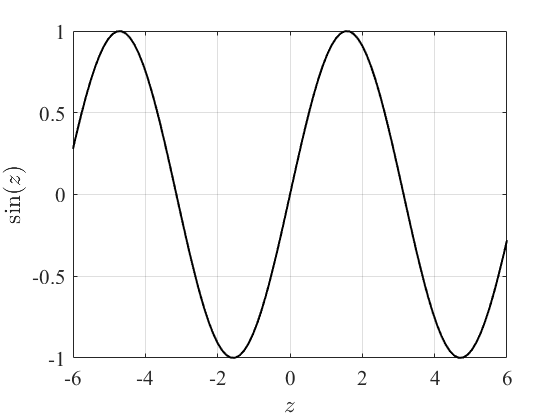
\includegraphics[width=0.35\textwidth]{Pictures/sin.png}
    \end{center}
    \caption[Graph of $\Phi$.]{Graph of $\Phi$ (unconstrained function).}
        \label{fig:sin example 1}
\end{figure}
\begin{figure}[ht!]
    \begin{center}
        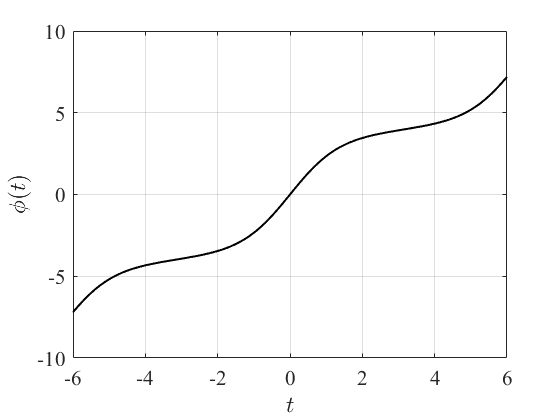
\includegraphics[width=0.35\textwidth]{Pictures/increased_sin.png}
    \end{center}
    \caption[Graph of $\phi = \mathcal{R}_{\mathrm{inc}}\{\Phi\}$.]{Graph of $\phi = \mathcal{R}_{\mathrm{inc}}\{\Phi\}$ (after first rectification).}
        \label{fig:sin example 2}
\end{figure}
\begin{figure}[ht!]
    \begin{center}
    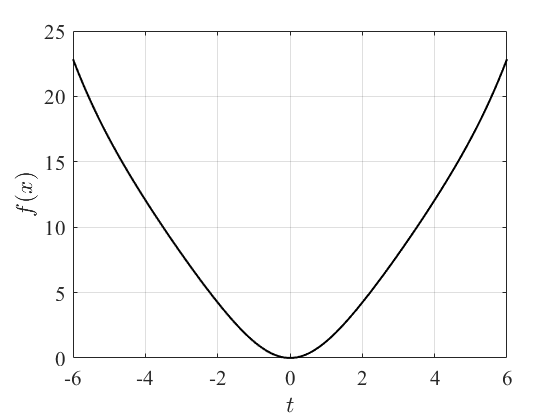
\includegraphics[width=0.35\textwidth]{Pictures/rectified_sin.png}
    \end{center}
    \caption[Graph of $f = \mathcal{R}_{\mathrm{cvx}}\{\phi\} = \mathcal{R}\{\Phi\}$.]{Graph of $f = \mathcal{R}_{\mathrm{cvx}}\{\phi\} = \mathcal{R}\{\Phi\}$ (fully rectified function).}
    \label{fig:sin example 3}
\end{figure}
Notice that in this example, the derivative of the rectified function $f$ cannot be required to vanish at an arbitrary point (as in Eq.~\eqref{eq:constraint-stationarity} for example), since the primary function $\Phi$ is fixed (as opposed to the case where it can be trained). 
\end{remark}


\section{Applications}\label{sec:applications}
We consider a standard setting where data are provided in the form stress-strain responses. For an incompressible material for instance, the Cauchy stress associated with the rectified NN is evaluated as
\begin{equation}
    {\bf\Sigma}^*(\bfF) = 2 {\bfF} \left(\sum_{i = 1}^{3} \frac{\partial w_i^*(I_i)}{ \partial I_i} \frac{\partial I_i}{ \partial \bfC} \right) \bfF^T - p\bfI\,,
\end{equation}
where the left-hand side depends on the parameters of the NN, $w_i^*$ is defined by Eq.~\eqref{eq:def-wistar}, $p$ is a Lagrange multiplier arising from the incompressibility condition (in practice, $p$ is evaluated by imposing a stress-free condition). 

Training with respect to data can be achieved using the cost function
\begin{equation}\label{eq:def-Ld}
     \mathcal{L}_d = \frac{\sum_{i = 1}^{N} \left( \Sigma^*(\bfF(\lambda_i)) - \Sigma^{\textnormal{data}}(\bfF(\lambda_i)) \right)^2}{\sum_{i = 1}^{N} \Sigma^{\textnormal{data}}(\bfF(\lambda_i))^2 }\,,
\end{equation}
along a loading path $\lambda \mapsto \bfF(\lambda)$, discretized with $N$ points. Here, $\Sigma^*$ denotes the relevant stress component (\textit{e.g.}, along testing direction), and $\{(\lambda_i, \Sigma^{\textnormal{data}}(\bfF(\lambda_i)))\}_{i = 1}^{N}$ constitutes the dataset. Note that the above loss function can be readily extended to cases where several loading conditions are considered (see Section \ref{subsec:exp-app}).

In the applications presented below, no attempt was made to fully optimize network architectures and training strategies. The numbers of layers and neurons per layer were determined through a standard parametric analysis on the validation loss defined by Eq.~\eqref{eq:def-Ld}. No activation function was used for the toy problem presented in Section \ref{subsec:toy}, while the sigmoid activation function was selected for all hidden layers in all other examples (in Sections \ref{subsec:MR}, \ref{subsec:anisotropic-app}, and \ref{subsec:exp-app}). 

The Adaptive Moment Estimation (ADAM) algorithm was used for training, with an implementation in JAX \cite{jax2018github}. 

\subsection{Toy Problem}\label{subsec:toy}
We first consider a toy example where the target convex function is given as
\begin{align}
        f^\textnormal{target}(x) = k_1 \exp\left( \frac{(x - k_2)^2}{2k_3^2} \right)\,, \quad \forall x \in \mathbb{R}\,,
\end{align}
where $k_1= 10$, $k_2= 5$, and $k_3= 20$. We seek to construct an approximation over the interval $I = [0, 10]$, centered without loss of generality around the abscissa $x = k_2$ at which $f^\textnormal{target}$ reaches its minimum, with $f(k_2) = k_1$. A set of $100$ equidistant data points is used for fitting, and 20 \% data points are used as the validation set. Adopting the generic notation $\psi$ for the neural network, the rectified model reads as
\begin{equation}
    f(x) = k_1 - \int_{0}^{k_2} \phi(t) \,dt + \int_{0}^x \phi(t) \,dt\,, \quad \forall x \in [0, 10]\,,
\end{equation}
where
\begin{equation}
    \phi(t) = \psi(0) + \int_{0}^t g\left(\frac{d\psi(z)}{dz}\right) \,dz\,.
\end{equation}
Three different choices for $g$ were considered, namely the square function $g(x) = x^2$, the exponential function $g(x) = \exp(x)$, and the modified soft-plus function $g(x) = \log(2^x+1)/\log(2)$. 

In this example, a simple neural network architecture with one hidden layer and two neurons is used (without activation functions). The learning rate for the ADAM optimizer is set to 0.01. Mean square validation errors for the rectified functions are reported in Tab.~\ref{tab:toy-problem-validation-errors} for the three choices of $g$. 
\begin{table}[ht!]
\centering
\begin{tabular}{|c|c|} 
 \hline
 Function $g$ & Error $\epsilon$ \\ 
 \hline
 Square & $1.5850 \times 10^{-7}$ \\ 
 \hline
 Exponential & $2.0018 \times 10^{-5}$ \\ 
 \hline
 Soft-plus & $1.6069 \times 10^{-7}$ \\ 
 \hline
 \end{tabular} 
\caption{Results for the validation step: $L^2$-norm errors for the rectified neural network model (toy problem).}
\label{tab:toy-problem-validation-errors}
\end{table}
The square and modified soft-plus functions provide fairly similar validation errors, smaller than the one obtained with the exponential function. In addition, the model rectified with the square function converged in 3,000 epochs, while the rectified model with the modified soft-plus function converged in about 8,000 epochs. The model with the exponential function converged in more than 10,000 epochs, which is slower than with the other two positive functions. In order to qualitatively assess the accuracy, the predictions obtained with the rectified neural network for the validation dataset are shown in Fig.~\ref{fig:toy-problem-qualitative-results} (see Tab.~\ref{tab:toy-problem-validation-errors} for validation metrics).
\begin{figure}[ht!]
    \begin{center}
        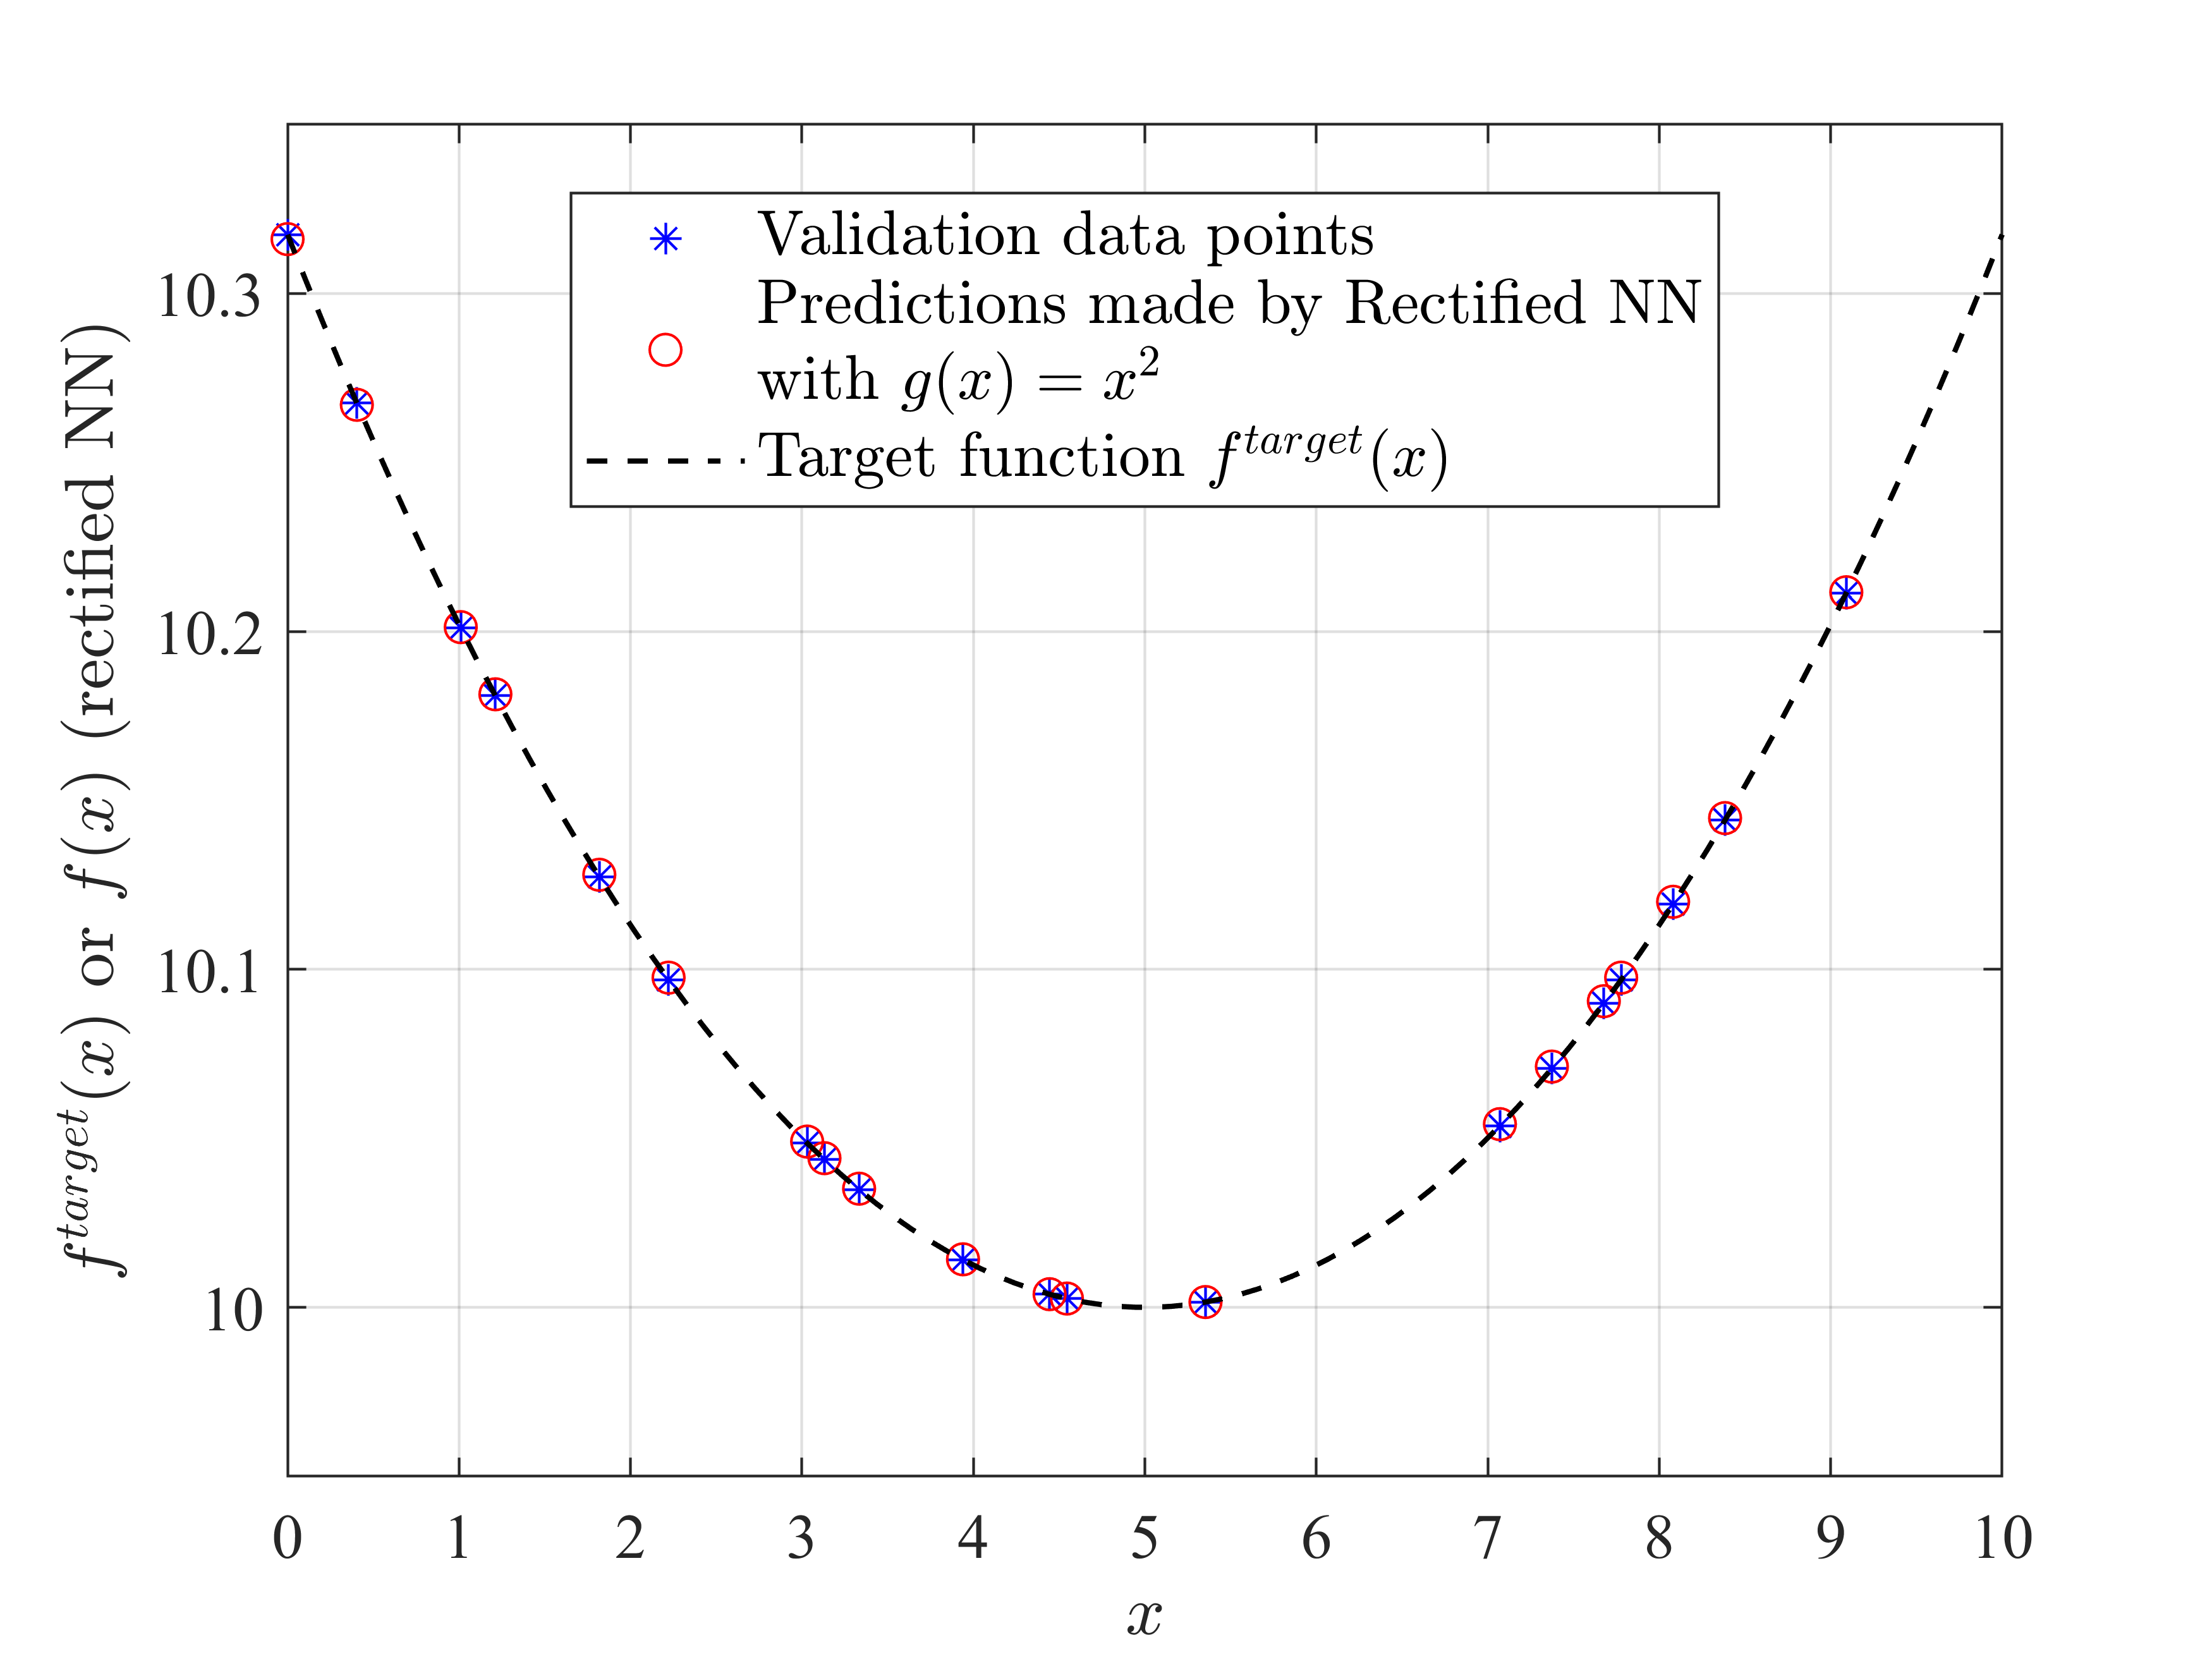
\includegraphics[width = 0.5\textwidth]{Pictures/toy.png}
    \end{center}
    \caption[Target function, reference values, and rectified neural network predictions.]{Target function (black dashed line), reference values (blue star), and rectified neural network predictions (red circles) for the validation dataset (random selection).}
    \label{fig:toy-problem-qualitative-results}
\end{figure}
Recall that no restrictions are imposed on weights and activation functions in the proposed formulation.

\subsection{Mooney-Rivlin Model}\label{subsec:MR}
Here we address the case of a Mooney–Rivlin material, defined by the stored energy function
\begin{equation}
    w{^\textnormal{MR}}(I_1,I_2) = C_1(I_1 - 3) + C_2(I_2 - 3)\,, \label{eq:MR}
\end{equation}
where $C_1$ and $C_2$ are strictly positive material parameters (see \cite{ciarlet1988mathematical}, p.~189). The rectified model is written as
\begin{equation}
    w^*(I_1, I_2) = w_1^*(I_1) + w_2^*(I_2)\,,
\end{equation}
with 
\begin{align}
    w_1^*(I_1) = \mathcal{R}\{\psi_1(\{\bfW_j^{(1)}, \bfb_j^{(1)}\}_{j = 1}^{n_1})\}(I_1)
\end{align}
and
\begin{align}
w_2^*(I_2) = \mathcal{R}\{\psi_2(\{\bfW_j^{(2)}, \bfb_j^{(2)}\}_{j = 1}^{n_2})\}(I_2)\,.
\end{align}
The Cauchy stress is given by (see \cite{HolzapfelBook}, p. 224)
\begin{equation}
    \boldsymbol{\Sigma} = 2C_1\bfB - 2C_2\bfB^{-1} - p \bfI\,.
\end{equation}
We consider uniaxial tension along the first direction for training purposes, in which case the uniaxial Cauchy stress writes 
\begin{equation}
    \Sigma(\lambda) = 2\left(C_1 + \frac{ C_2}{\lambda}\right)\left(\lambda^2 - \frac{1}{\lambda}\right)\,, \label{eq:MR_Cauchy}
\end{equation}
where $\lambda$ is the driving principal stretch. The uniaxial Cauchy stress associated with the rectified model can be evaluated as
\begin{equation}
    \Sigma^*(\lambda) = 2 \left( \frac{\partial w_1^*(I_1)}{\partial I_1} + \frac{\partial w_2^*(I_2)}{\partial I_2} \frac{1}{\lambda} \right) \left( \lambda^2 - \frac{1}{\lambda} \right)\,, 
\end{equation}
with
\begin{equation}
    \frac{\partial w_i^*(I_i)}{\partial I_i} =  \left( \psi_i(0) + \int_0^{I_i} g\left(\frac{d\psi_i}{dz}\right)\, dz \right)\,.
\end{equation}
Derivatives are computed using automatic differentiation. In this example, we consider an approximation for $\lambda \in [1.0, 1.4]$ ($I_1 \geq 3$ and $I_2 \geq 3$). The material parameters are arbitrarily chosen as $C_1 = 10$ and $C_2 = 5$. Normalization condition is imposed by taking $w_1^*(3) = w_2^*(3) = 0$ with the constant terms (see Eq.~\eqref{eq:Rec-Con}, with $a = 3$) set to 0. Note that the stress free condition is automatically satisfied owing to the definition of $p$.

Two hundreds datapoints are generated using Eq.~\eqref{eq:MR_Cauchy}, with 20 \% of samples allocated for validation.  Parametric studies on validation error were conducted to identify the NN architecture, using a learning rate set to $0.01$, 5,000 epochs, and the square function (in the first rectifier); see Fig.~\ref{fig:Mr_Err_Study}.
\begin{figure}[ht!]
    \begin{center}
        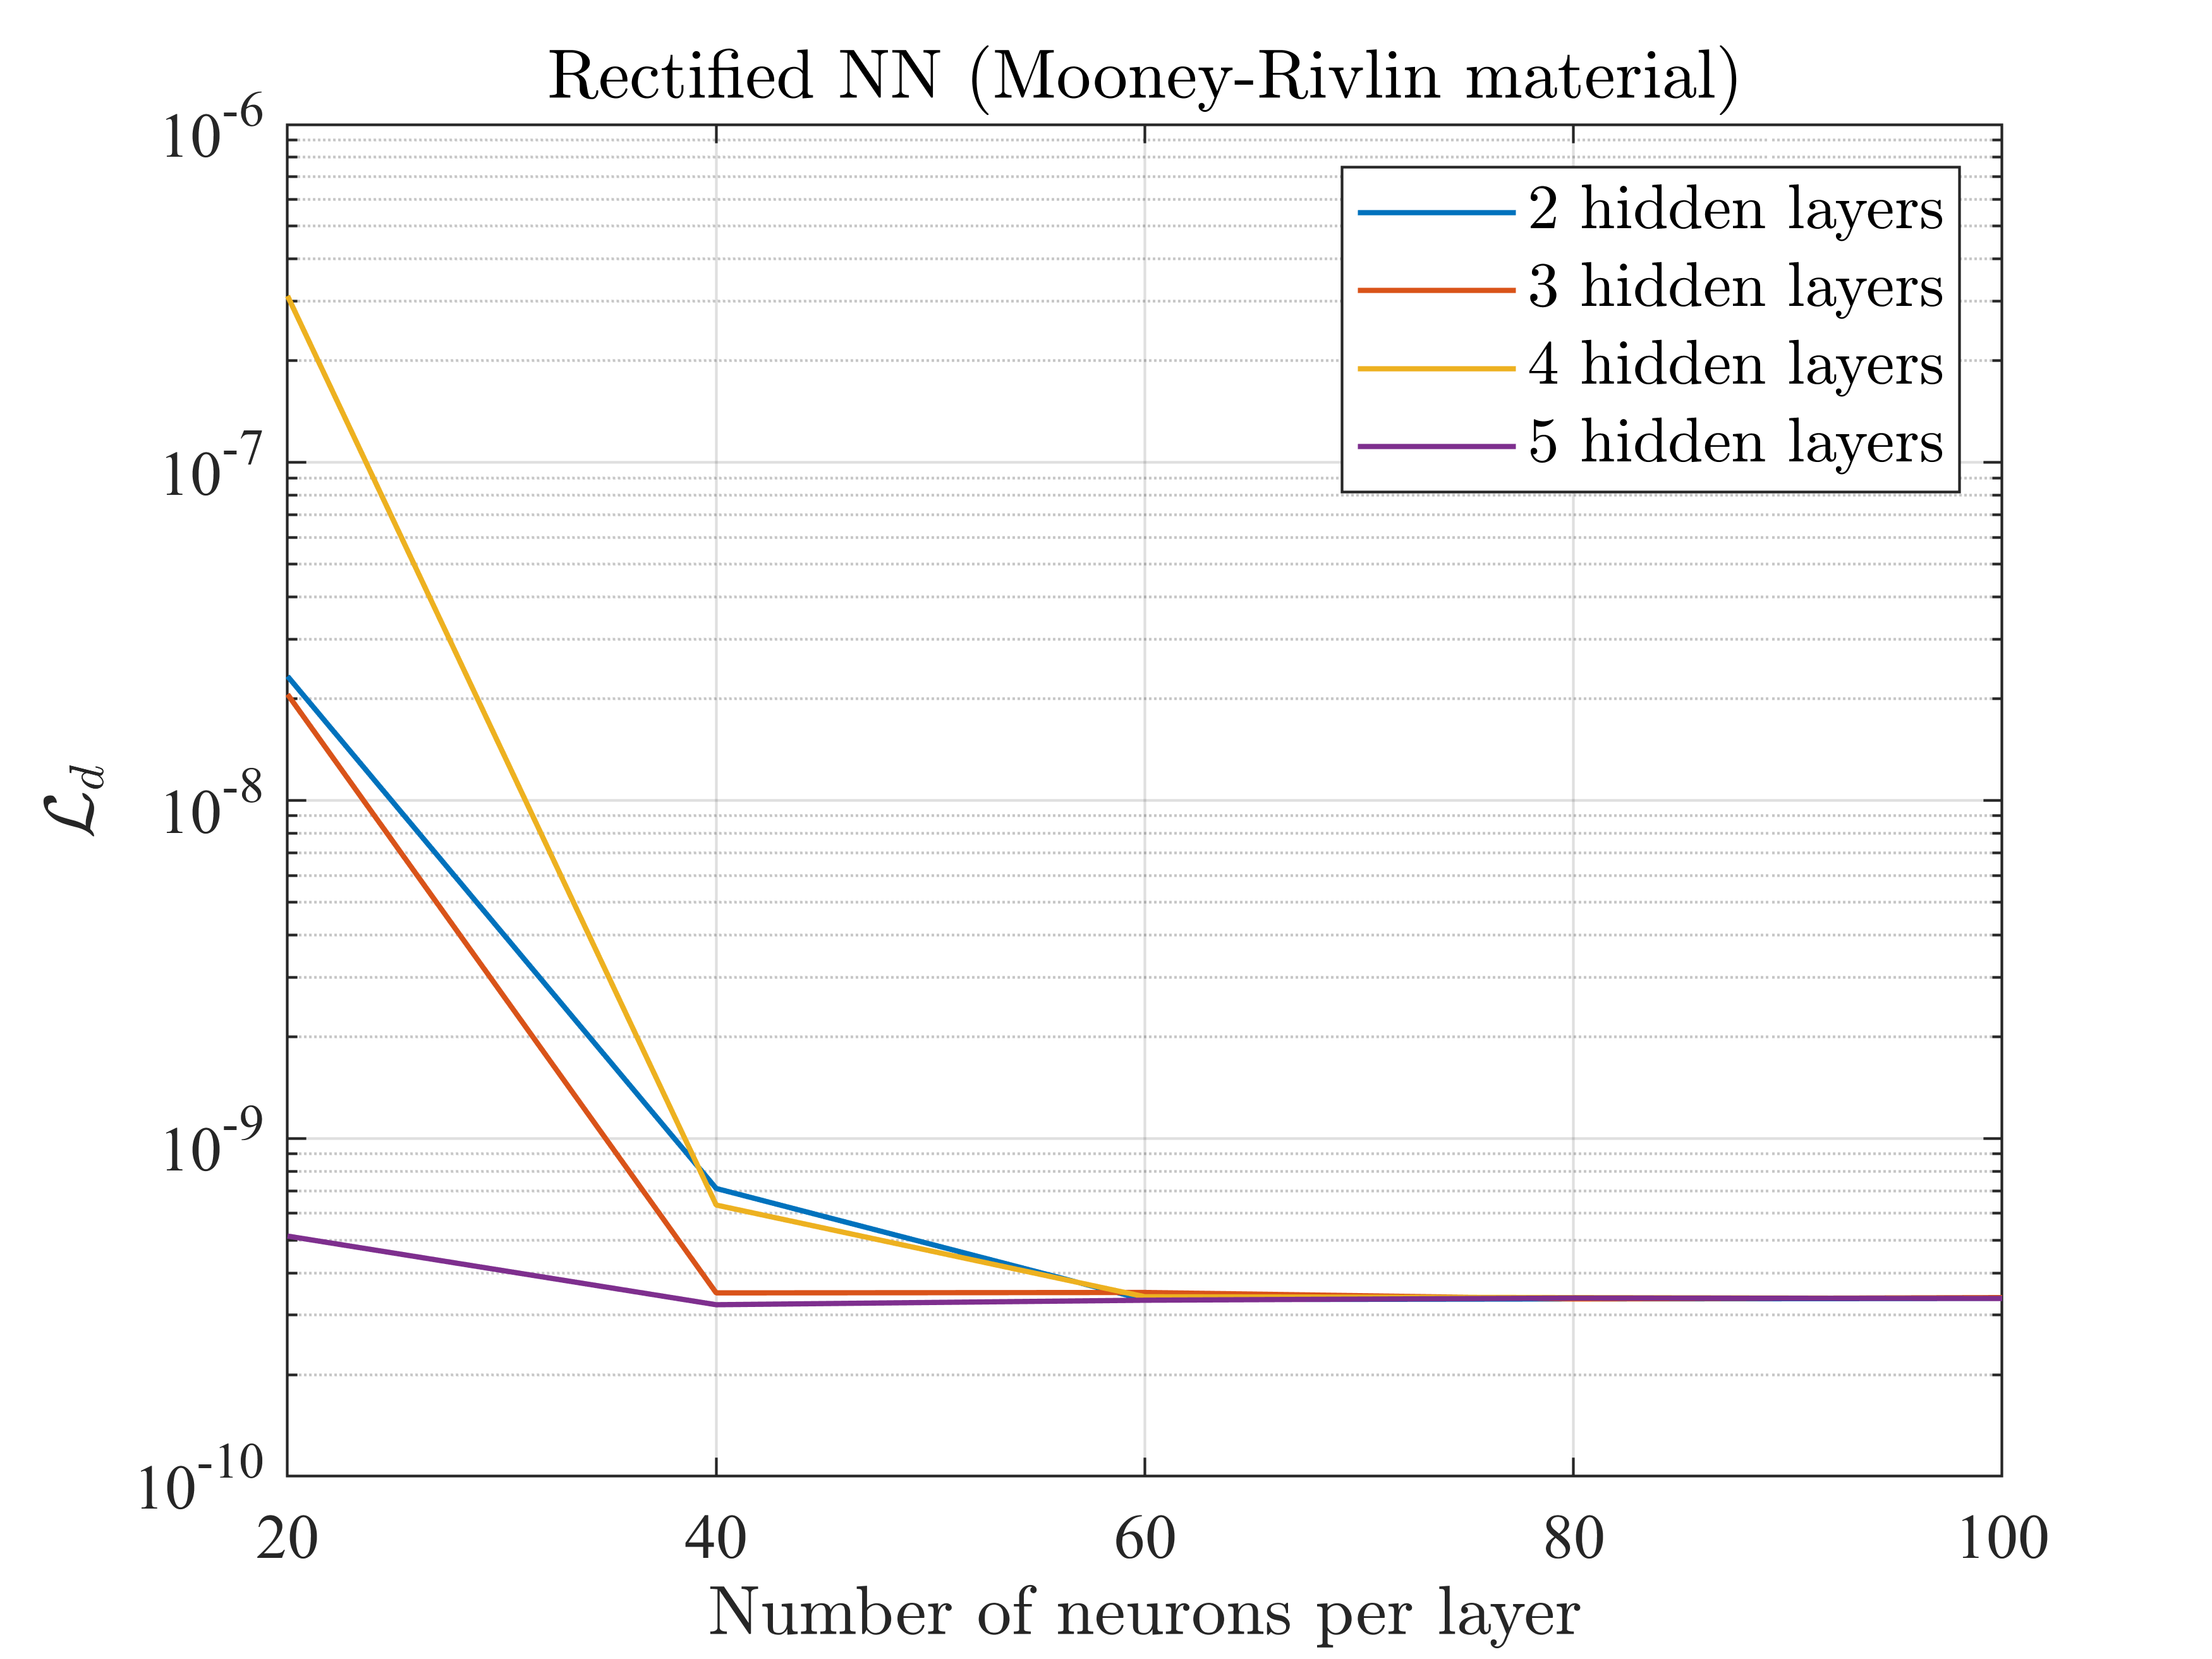
\includegraphics[width = 0.5\textwidth]{Pictures/Mr_Err.png}
    \end{center}
    \caption{Loss function $\mathcal{L}_d$ for different neural network architectures on the validation dataset (Mooney-Rivlin material).}
    \label{fig:Mr_Err_Study} 
\end{figure}
Results predicted by the calibrated rectified neural network model (with 5 layers and 40 neurons per layer) on the validation dataset is shown in Fig.~\ref{fig:MR best result 1}.
\begin{figure}[ht!]
    \begin{center}
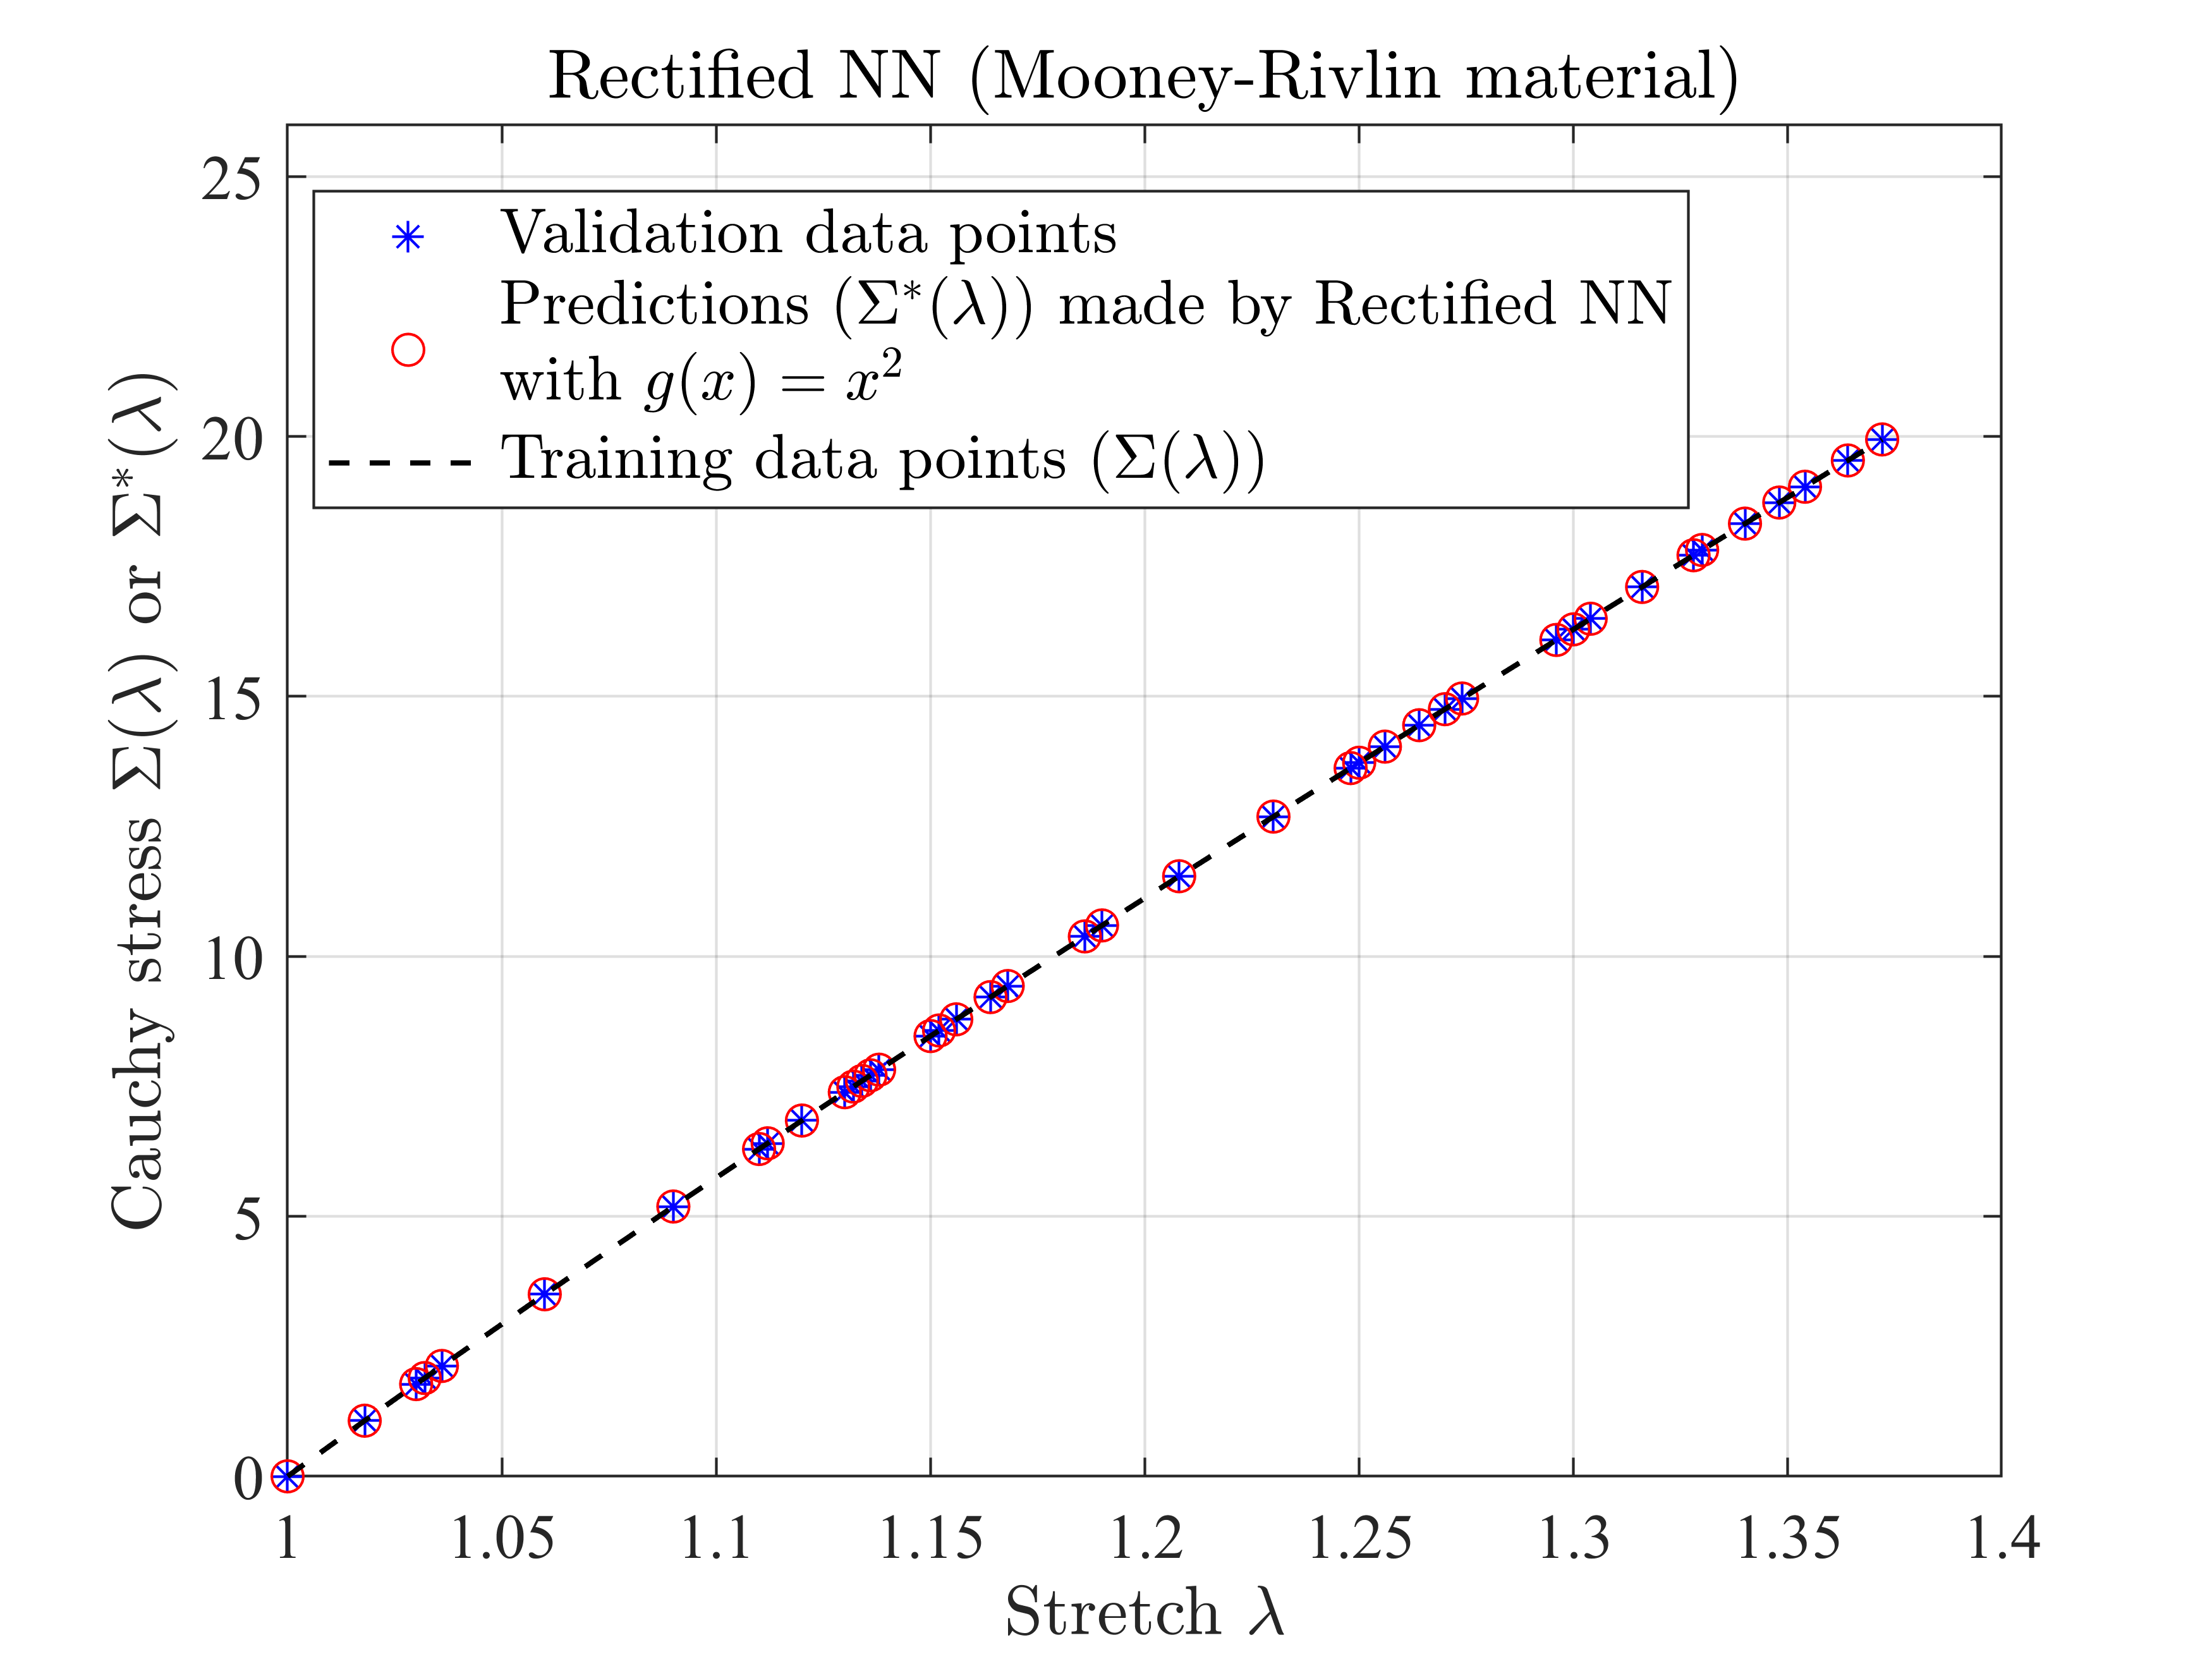
\includegraphics[width=0.5\textwidth]{Pictures/sigma_MR.png}
    \end{center}
    \caption{Reference stress response $\lambda \mapsto \Sigma(\lambda)$ (black dashed line), reference values (blue star), and rectified neural network predictions (red circle) for the validation dataset (random selection). Here, 5 hidden layers and 40 neurons per layer are used.}
    \label{fig:MR best result 1}
\end{figure}

\begin{remark} As indicated in Section \ref{sec:intro}, Input-Convex Neural Networks (ICNNs) can be obtained by forcing all weights, except those connected to the input, to be non-negative, and by using only convex non-decreasing activation functions \cite{amos2017input, as2022mechanics,Asad-IJNME,KLEIN2022104703}. In order to evaluate the performance of such constrained neural networks in terms of training results, we consider a model of the form 
\begin{align}
    \psi_{\mathrm{ICNN}}(I_1, I_2) &= \psi_{\mathrm{ICNN}}^{(1)}(I_1) + \psi_{\mathrm{ICNN}}^{(2)}(I_2)\,,
\end{align}
where each ICNN involves unconstrained weights that are mapped to positive weights in the loss function, using the modified soft-plus activation function proposed in \cite{as2022mechanics,Asad-IJNME}. The validation loss history for each approach is shown in Fig.\ref{fig:ERR_history} for the Mooney-Rivlin dataset.
\begin{figure}[ht!]
    \begin{center}
        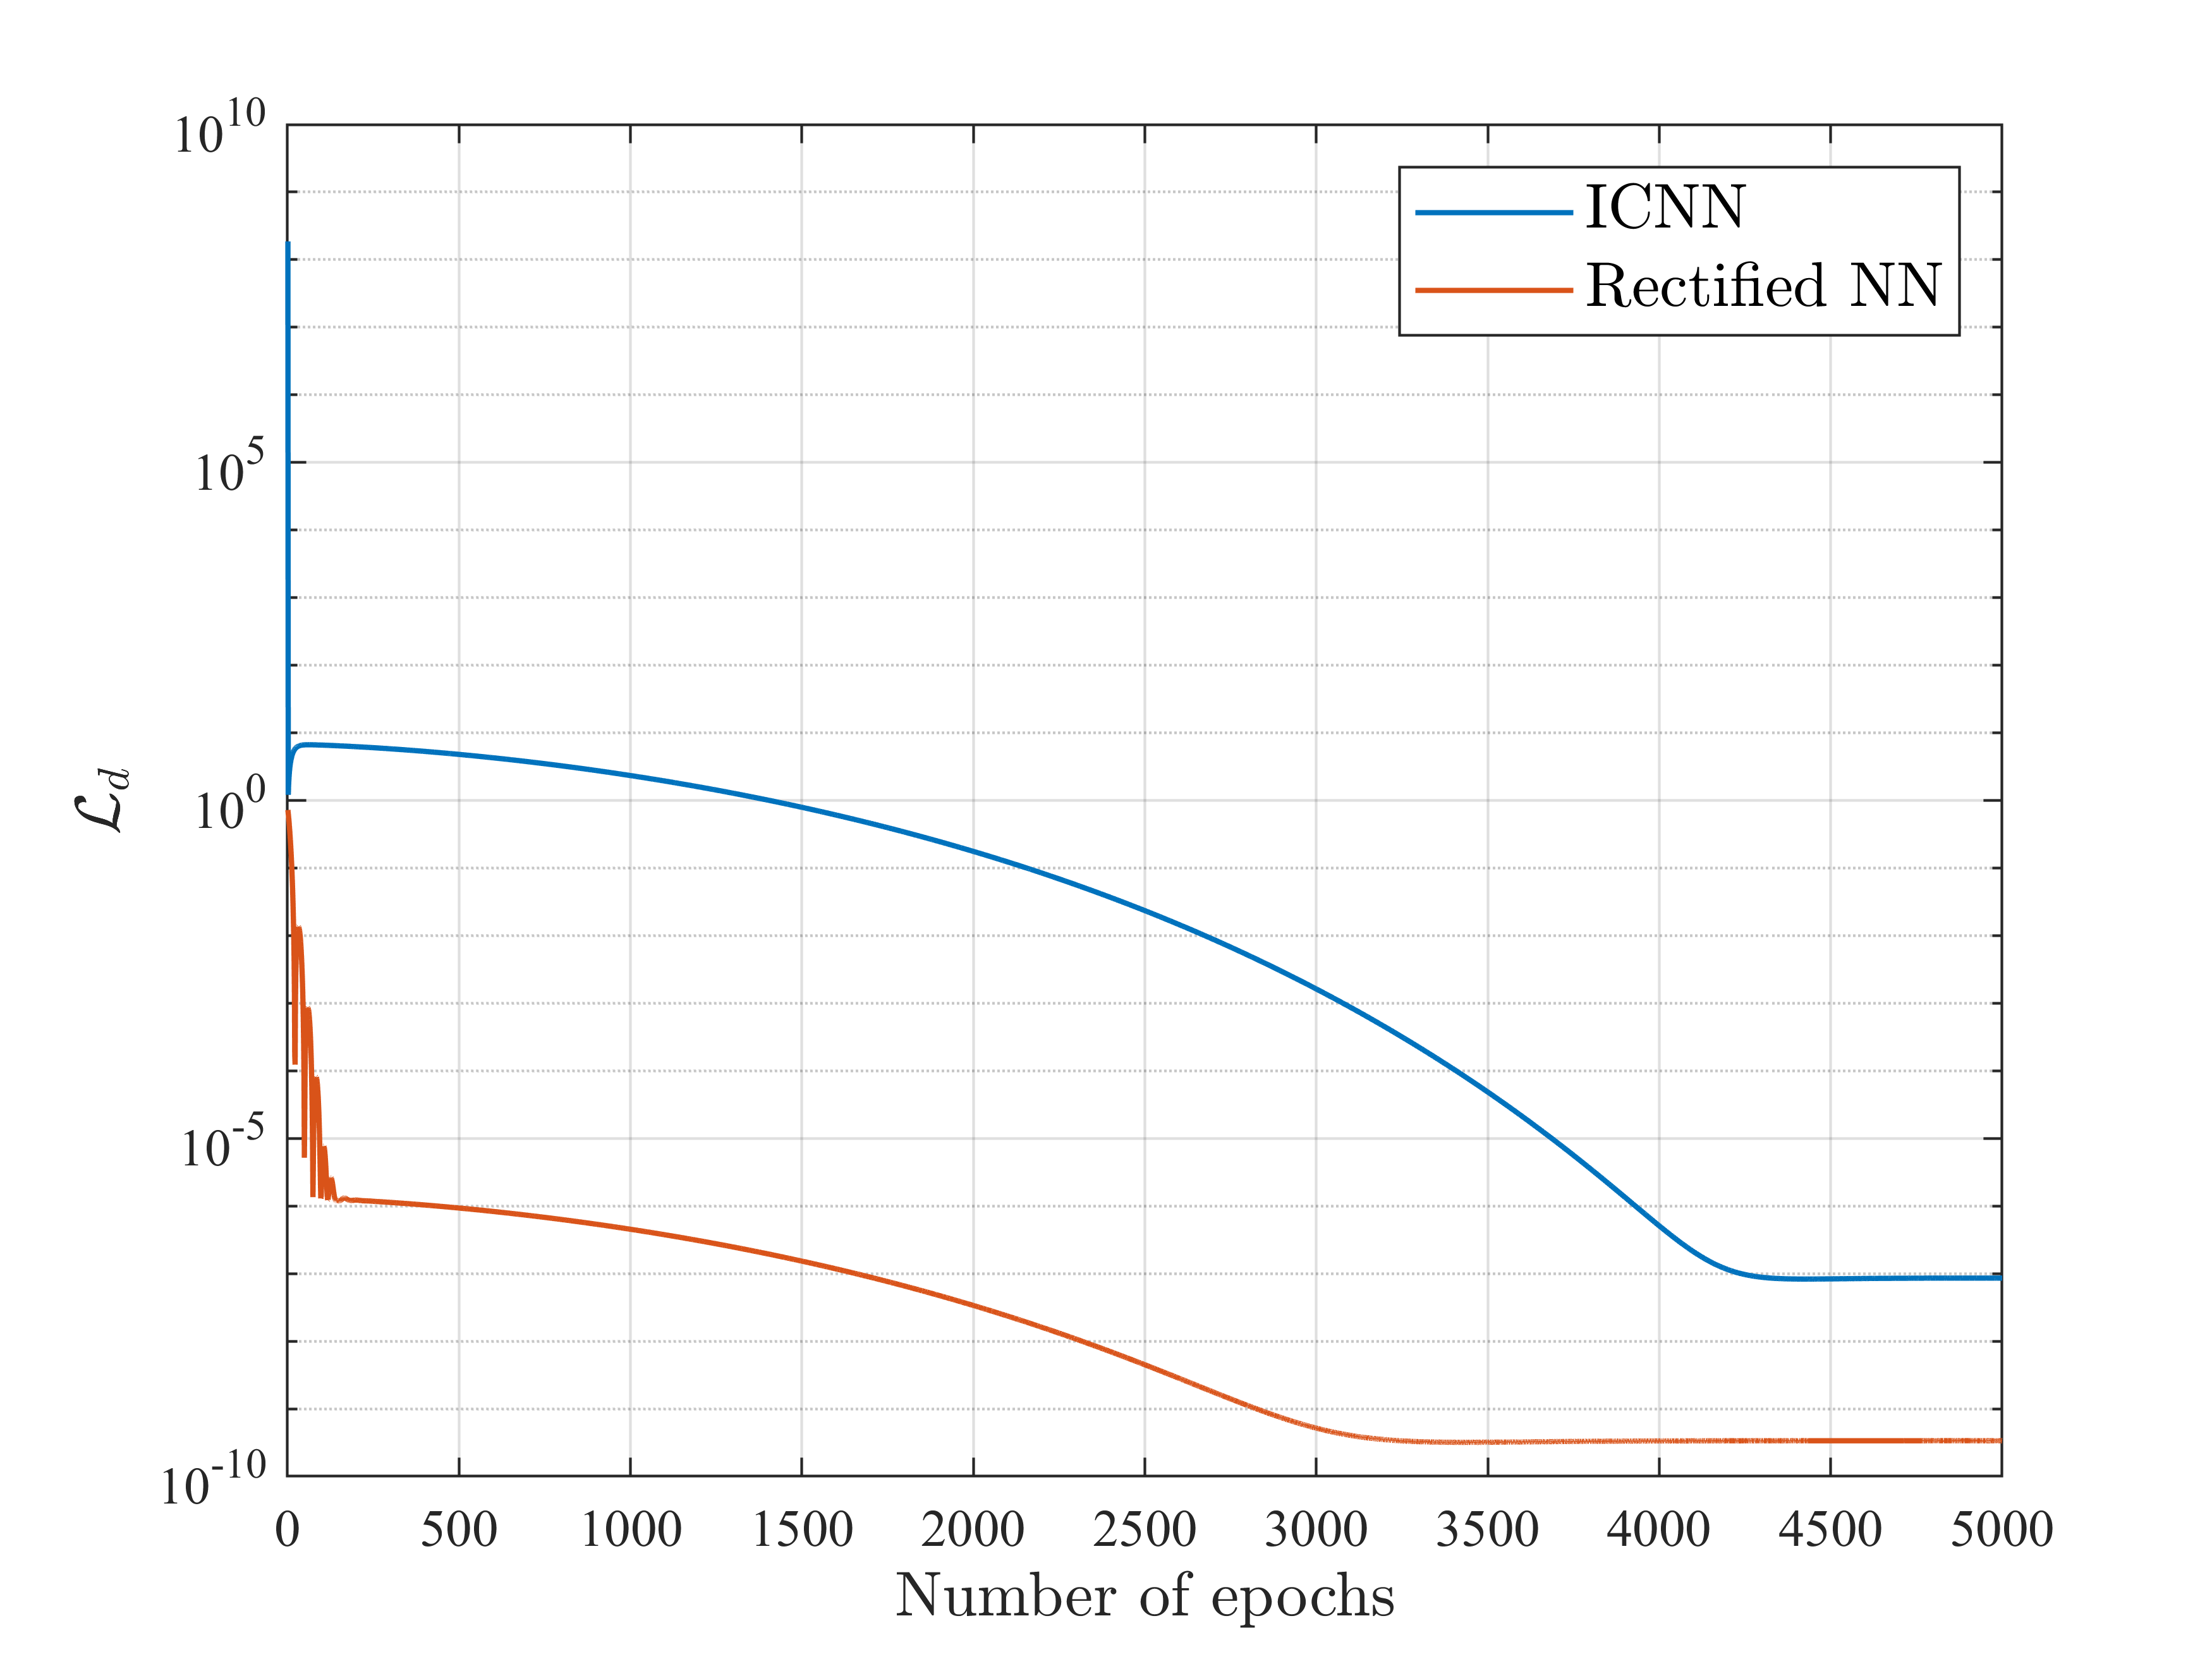
\includegraphics[width = 0.5\textwidth]{Pictures/loss_hist.png}
    \end{center}
    \caption[Loss history for ICNN and the proposed rectified NN.]{Loss history for ICNN and the proposed rectified NN.}
    \label{fig:ERR_history} 
\end{figure}
Reported results were obtained with 2 hidden layers and 20 neurons per layer for both strategies, based on a parametric convergence study on the validation metric. It is seen that the rectified NN converges much faster than the ICNN and leads to a lower training error. While similar results were obtained for a wide range of architectures, it should be pointed out that the computational cost per iteration is greater in the case of rectified NNs, which require numerical integration to be performed. In addition, opposite trends with respect to learning rates were observed: ICNNs tend to perform slightly better at large learning rates (\textit{e.g.}, 1.5) but require a very large number of iterations (greater than 40,000) at standard learning rates (\textit{e.g.}, 0.001). These observations are most likely imputable to the transformation of negative weights, which generates large regions with ``flat'' gradients in the optimization process. In contrast, rectified NNs were found to perform steadily in terms of training cost, regardless of the learning rate, and typically performs (much) better at smaller rates. An extensive comparison of the tradeoffs between these approaches is left for future work.
\end{remark}

\subsection{Anisotropic Model for Digital Dataset} \label{subsec:anisotropic-app}
We next consider an anisotropic strain energy density function, relevant to the modeling of soft biological tissues such as arterial vessels \cite{balzani2006polyconvex,staber2018stochastic}. It should be noticed such materials are often modeled as nearly-incompressible in a computational setting, in which case the strain energy density function is typically expressed in terms of isochoric invariants. The reference function is defined as
\begin{equation}
    w(I_1, I_2, J_4^{(1)}, J_4^{(2)}) = w{^\textnormal{MR}}(I_1,I_2) + w{^\textnormal{A}}(J_4^{(1)}, J_4^{(2)})\,,
\end{equation}
where $w{^\textnormal{MR}}$ is given by Eq.~\eqref{eq:MR} and the anisotropic term is defined as
\begin{equation}
    w{^\textnormal{A}}(J_4^{(1)}, J_4^{(2)}) = \sum_{k=1}^2 w^{\text{ti}} (J_4^{(k)})\,,
\end{equation}
with
\begin{align}
    w^{\text{ti}} (J_4^{(k)}) = \frac{\mu_4}{\beta_4} \left\{ \exp \left(\beta_4 w^B(I_1, J_4^{(k)}) \right) - 1\right\} \label{eq: psi tissue}
\end{align}
where $w^B(I_1, J_4^{(k)}) = (1-\rho)(I_1 - 3)^2 + \rho \langle J_4^{(k)} - 1 \rangle_m^2$, and $J_4^{(k)}= \tr(\bfC \bfM^{(k)})$. The structural tensors $\bfM^{(k)} = \bfa^{(k)} \otimes \bfa^{(k)}$ are defined in terms of the unit vectors 
\begin{subequations}
    \begin{align}
        \bfa^{(1)} &= \cos(\alpha) \bfe^{(1)} + \sin(\alpha)\bfe^{(2)}\,, \\ 
        \bfa^{(2)} &= \cos(\alpha) \bfe^{(1)} - \sin(\alpha)\bfe^{(2)}\,,
    \end{align}
\end{subequations}
where $\bfe^{(1)}$ and $\bfe^{(2)}$ are unit basis vectors and $\alpha$ is the angle defining the directions of anisotropy. In Eq.~\eqref{eq: psi tissue}, $\mu_4$, $\beta_4$, and $\rho$ are material parameters, and $\langle \cdot \rangle_m$ denotes the Macaulay bracket. Note that the angle $\alpha$ is also considered as a trainable parameter.

The rectified neural network is sought as
\begin{equation}\label{eq:rec-model-anisotropic-case}
    w_1^*(I_1) + w_2^*(I_2) + w_3^*(J_4^{(1)}) + w_4^*(J_4^{(2)})\,,
\end{equation}
where
\begin{equation}
    w_i^*(I_i) = \mathcal{R}\{\psi_i(\{\bfW_j^{(i)}, \bfb_j^{(i)}\}_{j = 1}^{n_i})\}(I_i)\,,\quad i=1,2\,,
\end{equation}
\begin{align}
    w_{3}^*(J_4^{(1)}) = \mathcal{R}\{\psi_3(\{\bfW_j^{(3)}, \bfb_j^{(3)}\}_{j = 1}^{n_3})\}(J_4^{(1)})\,,
\end{align}
and
\begin{align}
    w_{4}^*(J_4^{(2)}) = \mathcal{R}\{\psi_4(\{\bfW_j^{(4)}, \bfb_j^{(4)}\}_{j = 1}^{n_4})\}(J_4^{(2)})\,.
\end{align}
Biaxial tension is used for training purposes. The Cauchy stress associated with the reference model is obtained as
\begin{align}
     \Sigma(\lambda) = \Sigma^{\text{MR}}(\lambda) + \Sigma_{(1)}^{\text{ti}} (\lambda) + \Sigma_{(2)}^{\text{ti}} (\lambda)\,,
\end{align}
with
\begin{equation}
    \Sigma^{\text{MR}}(\lambda) = 2C_1(\lambda^2 - \frac{1}{\lambda^4}) - 2C_2(\frac{1}{\lambda^2} - \lambda^4)\,,
\end{equation}
and
\begin{align}
    \Sigma^{\text{ti}}_{(k)}(\lambda) = & \, 4 \lambda^2 \mu_4 \left\{ (1-\rho)(I_1 - 3)\left(1 - \frac{1}{\lambda^6}\right) \right.  \nonumber \\
    & \quad + \left. \rho \langle J_4^{(k)} - 1 \rangle_m \cos^2(\alpha) \right\}  \nonumber\\
    &\quad \times \exp(\beta_4 w^B(I_1, J_4^{(k)}))\,, \quad k = 1,2\,.
\end{align}
with a slight abuse of notation. The Cauchy stress for the rectified model defined by Eq.~\eqref{eq:rec-model-anisotropic-case} is given by
\begin{align}\label{eq:ANI_Cauchy}
    \Sigma^{*} = \Sigma^*_1(\lambda) + \Sigma^*_2(\lambda) +  \Sigma^*_3(\lambda) + \Sigma^*_4(\lambda)\,,
\end{align}
where terms in the right-hand side are defined as $\Sigma^*_1(\lambda) = 2 \frac{\partial w_1^*(I_1)}{\partial I_1} \left( \lambda^2 - \frac{1}{\lambda^4} \right)$, 
\begin{equation}
    \Sigma^*_1(\lambda) = 2 \frac{\partial w_1^*(I_1)}{\partial I_1} \left( \lambda^2 - \frac{1}{\lambda^4} \right)\,, 
\end{equation}
\begin{equation}
    \Sigma^*_2(\lambda) = -2 \frac{\partial w_2^*(I_2)}{\partial I_2} \left(\frac{1}{\lambda^2} - \lambda^4 \right)\,,
\end{equation}
\begin{equation}
    \Sigma_3^*(\lambda) = 2 \lambda^2 \frac{\partial w_3^*(J_4^{(1)})}{\partial J_4^{(1)}} \cos^2(\alpha)\,,
\end{equation}
\begin{equation}\label{eq:aniso-last-stress-component}
    \Sigma_4^*(\lambda) = 2 \lambda^2 \frac{\partial w_4^*(J_4^{(2)})}{\partial J_4^{(2)}} \cos^2(\alpha)\,.
\end{equation}
Since $\cos(\alpha) \neq 0$ in practice, the stress free constraint reduces to $\Sigma^*_3(1) + \Sigma^*_4(1) = 0$.
% \begin{align}\label{eq:stress-free-constraint-anisotropic-model}
%     \Sigma^*_3(1) + \Sigma^*_4(1) = 0\,.
% \end{align}
In the numerical example below, the material parameters correspond to the values identified in \cite{CHEN2022114897} for sample \#10 in the media layer: $C_1 = 0.7071$ [kPa], $C_2 = 0.0531$ [kPa], $\alpha = 0.2740$ [rad], $\mu_4 = 15.5753$ [kPa], $\beta_4 = 2.5561$, and $\rho = 0.0986$. Similarly to the previous case, we generated 200 datapoints, 20\% of which are used as the validation set. The learning rate is set to 0.005 for the first 3,000 epochs and then to 0.001 for 3,000 epochs, and presented results were obtained using the exponential function in the rectifier (i.e., $g(x) = \exp(x)$). The validation errors for different neural network architectures are shown in Fig.~\ref{fig:ani_err}.
\begin{figure}[ht!]
    \begin{center}
    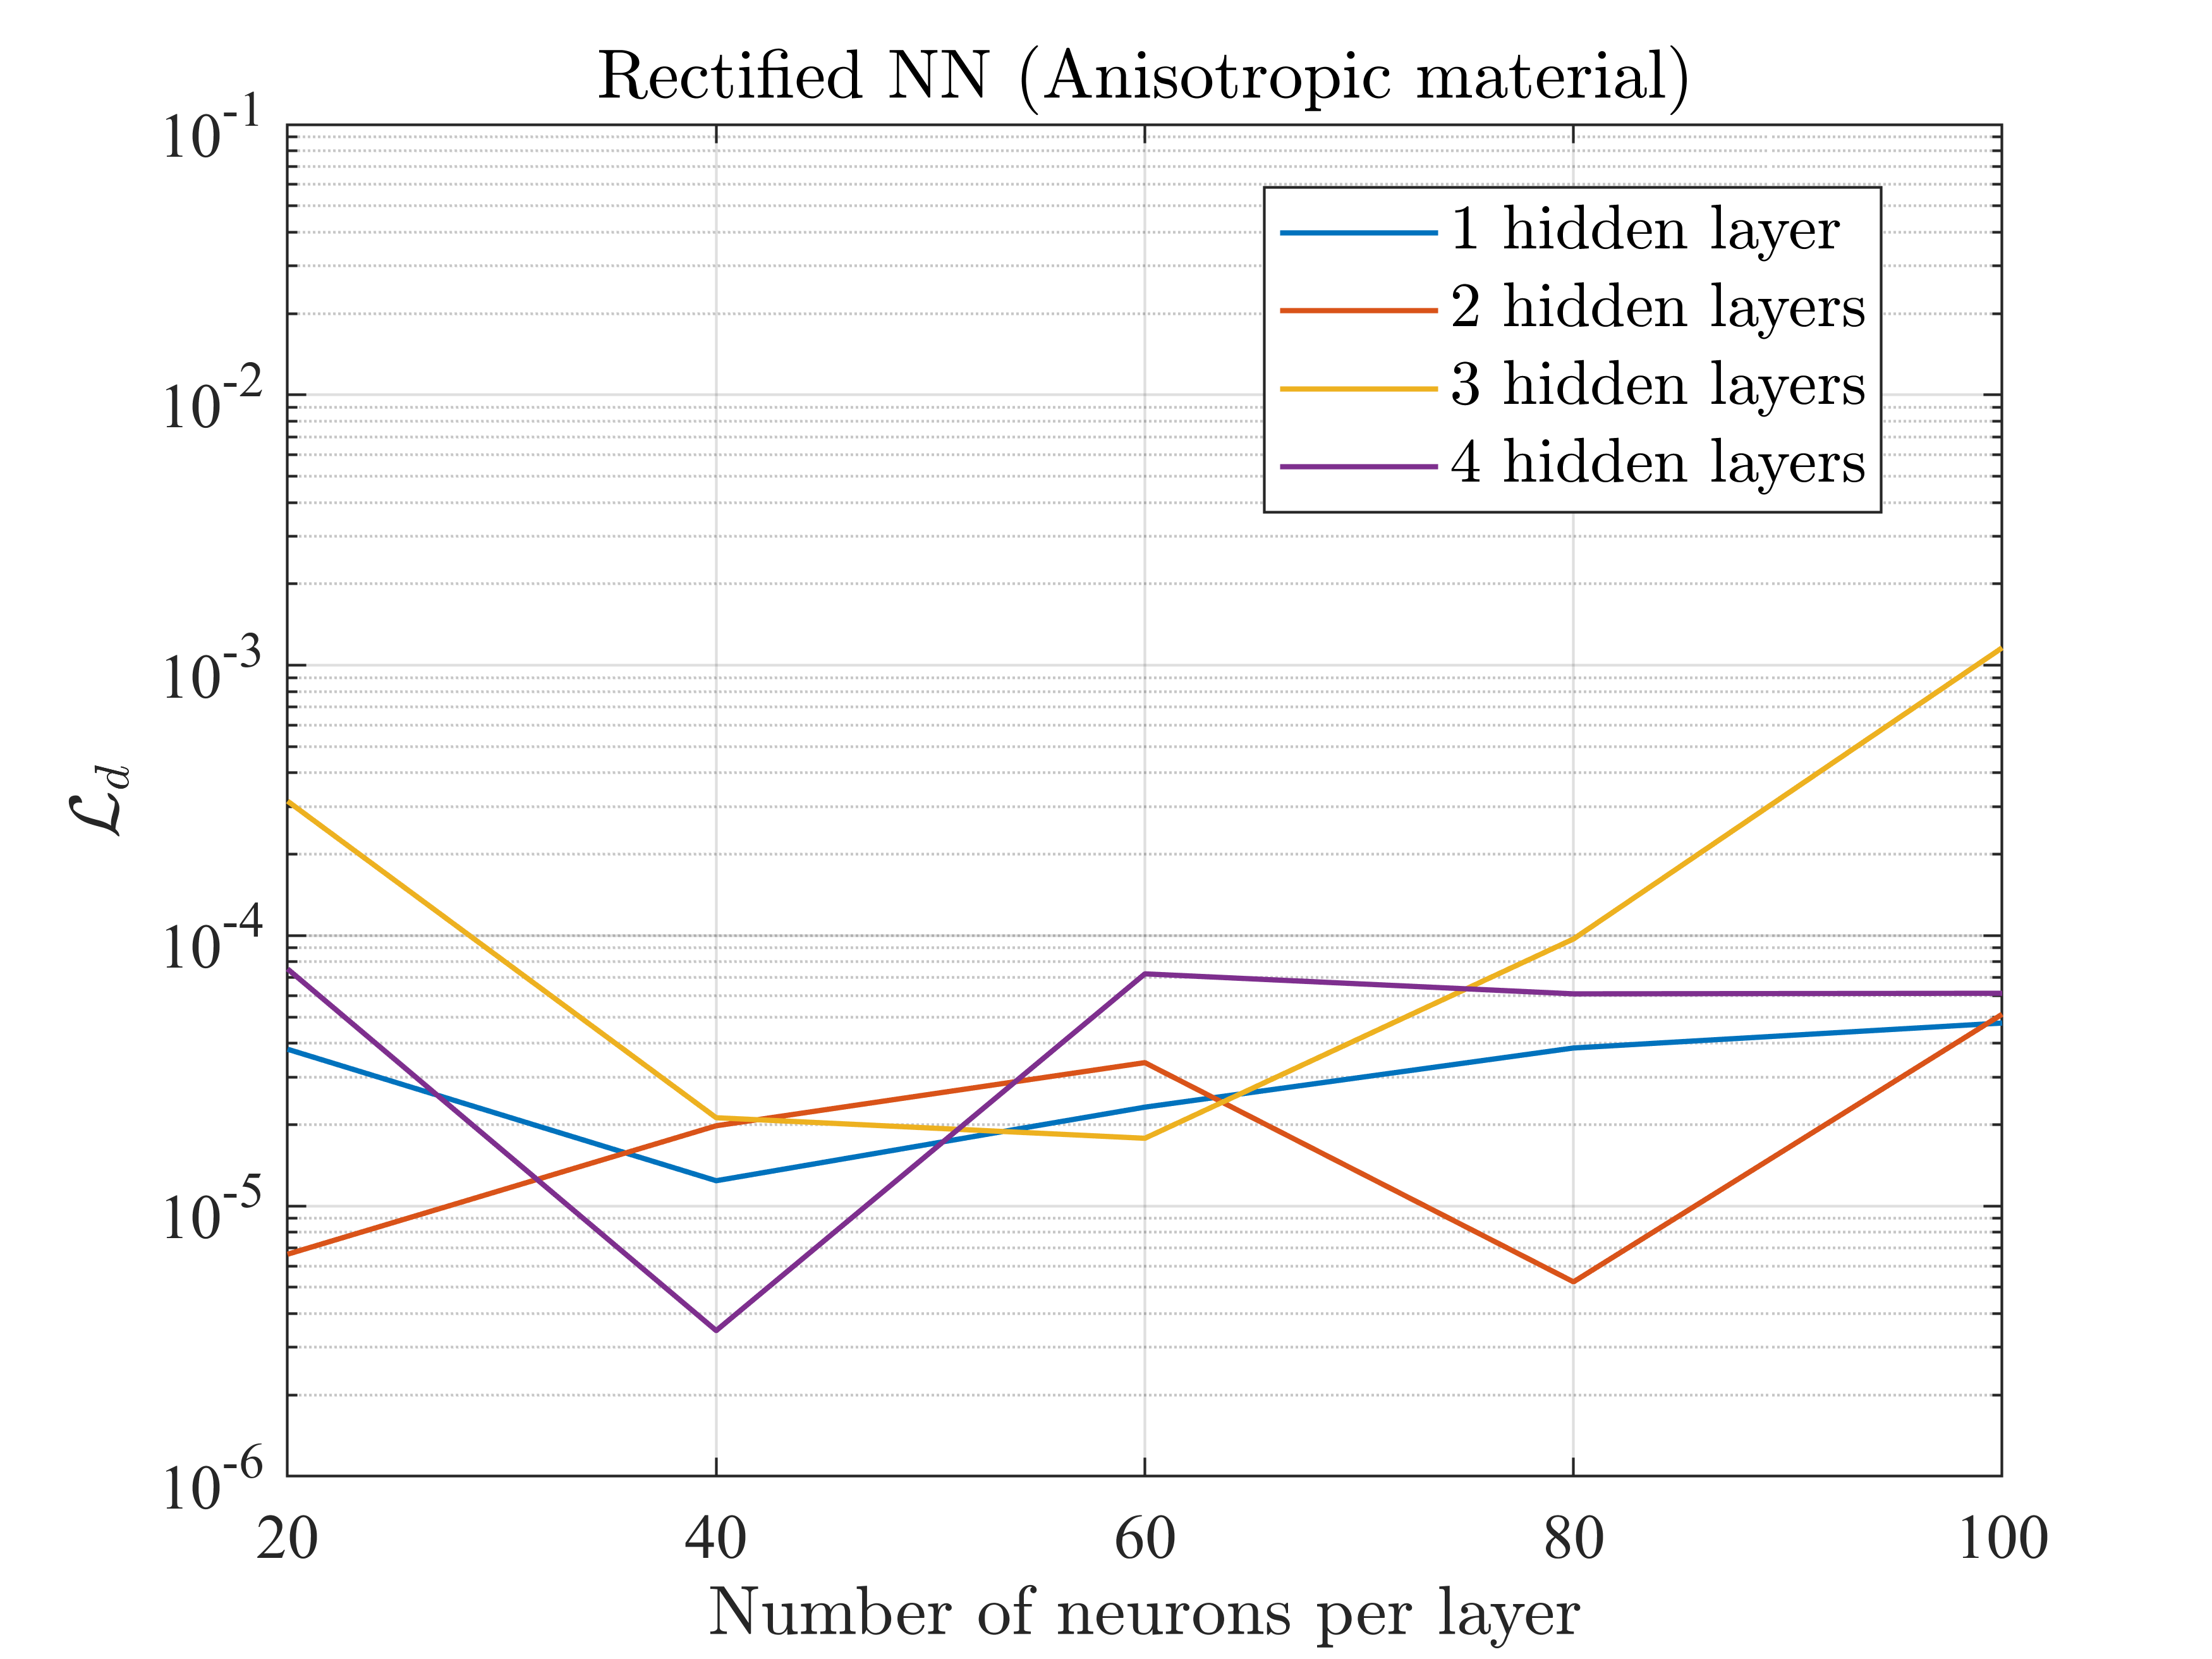
\includegraphics[width=0.5\textwidth]{Pictures/ANI_ERR.png}
    \end{center}
    \caption[Parametric study for different NN architectures.]{Parametric study of the mean squared error for different NN architectures on the validation dataset (Anisotropic material).}
    \label{fig:ani_err}
\end{figure}
Results predicted with the fitted rectified neural network model on the validation dataset are shown in Figs.~\ref{fig:ANI best result 1}.
\begin{figure}[ht!]
    \begin{center}
        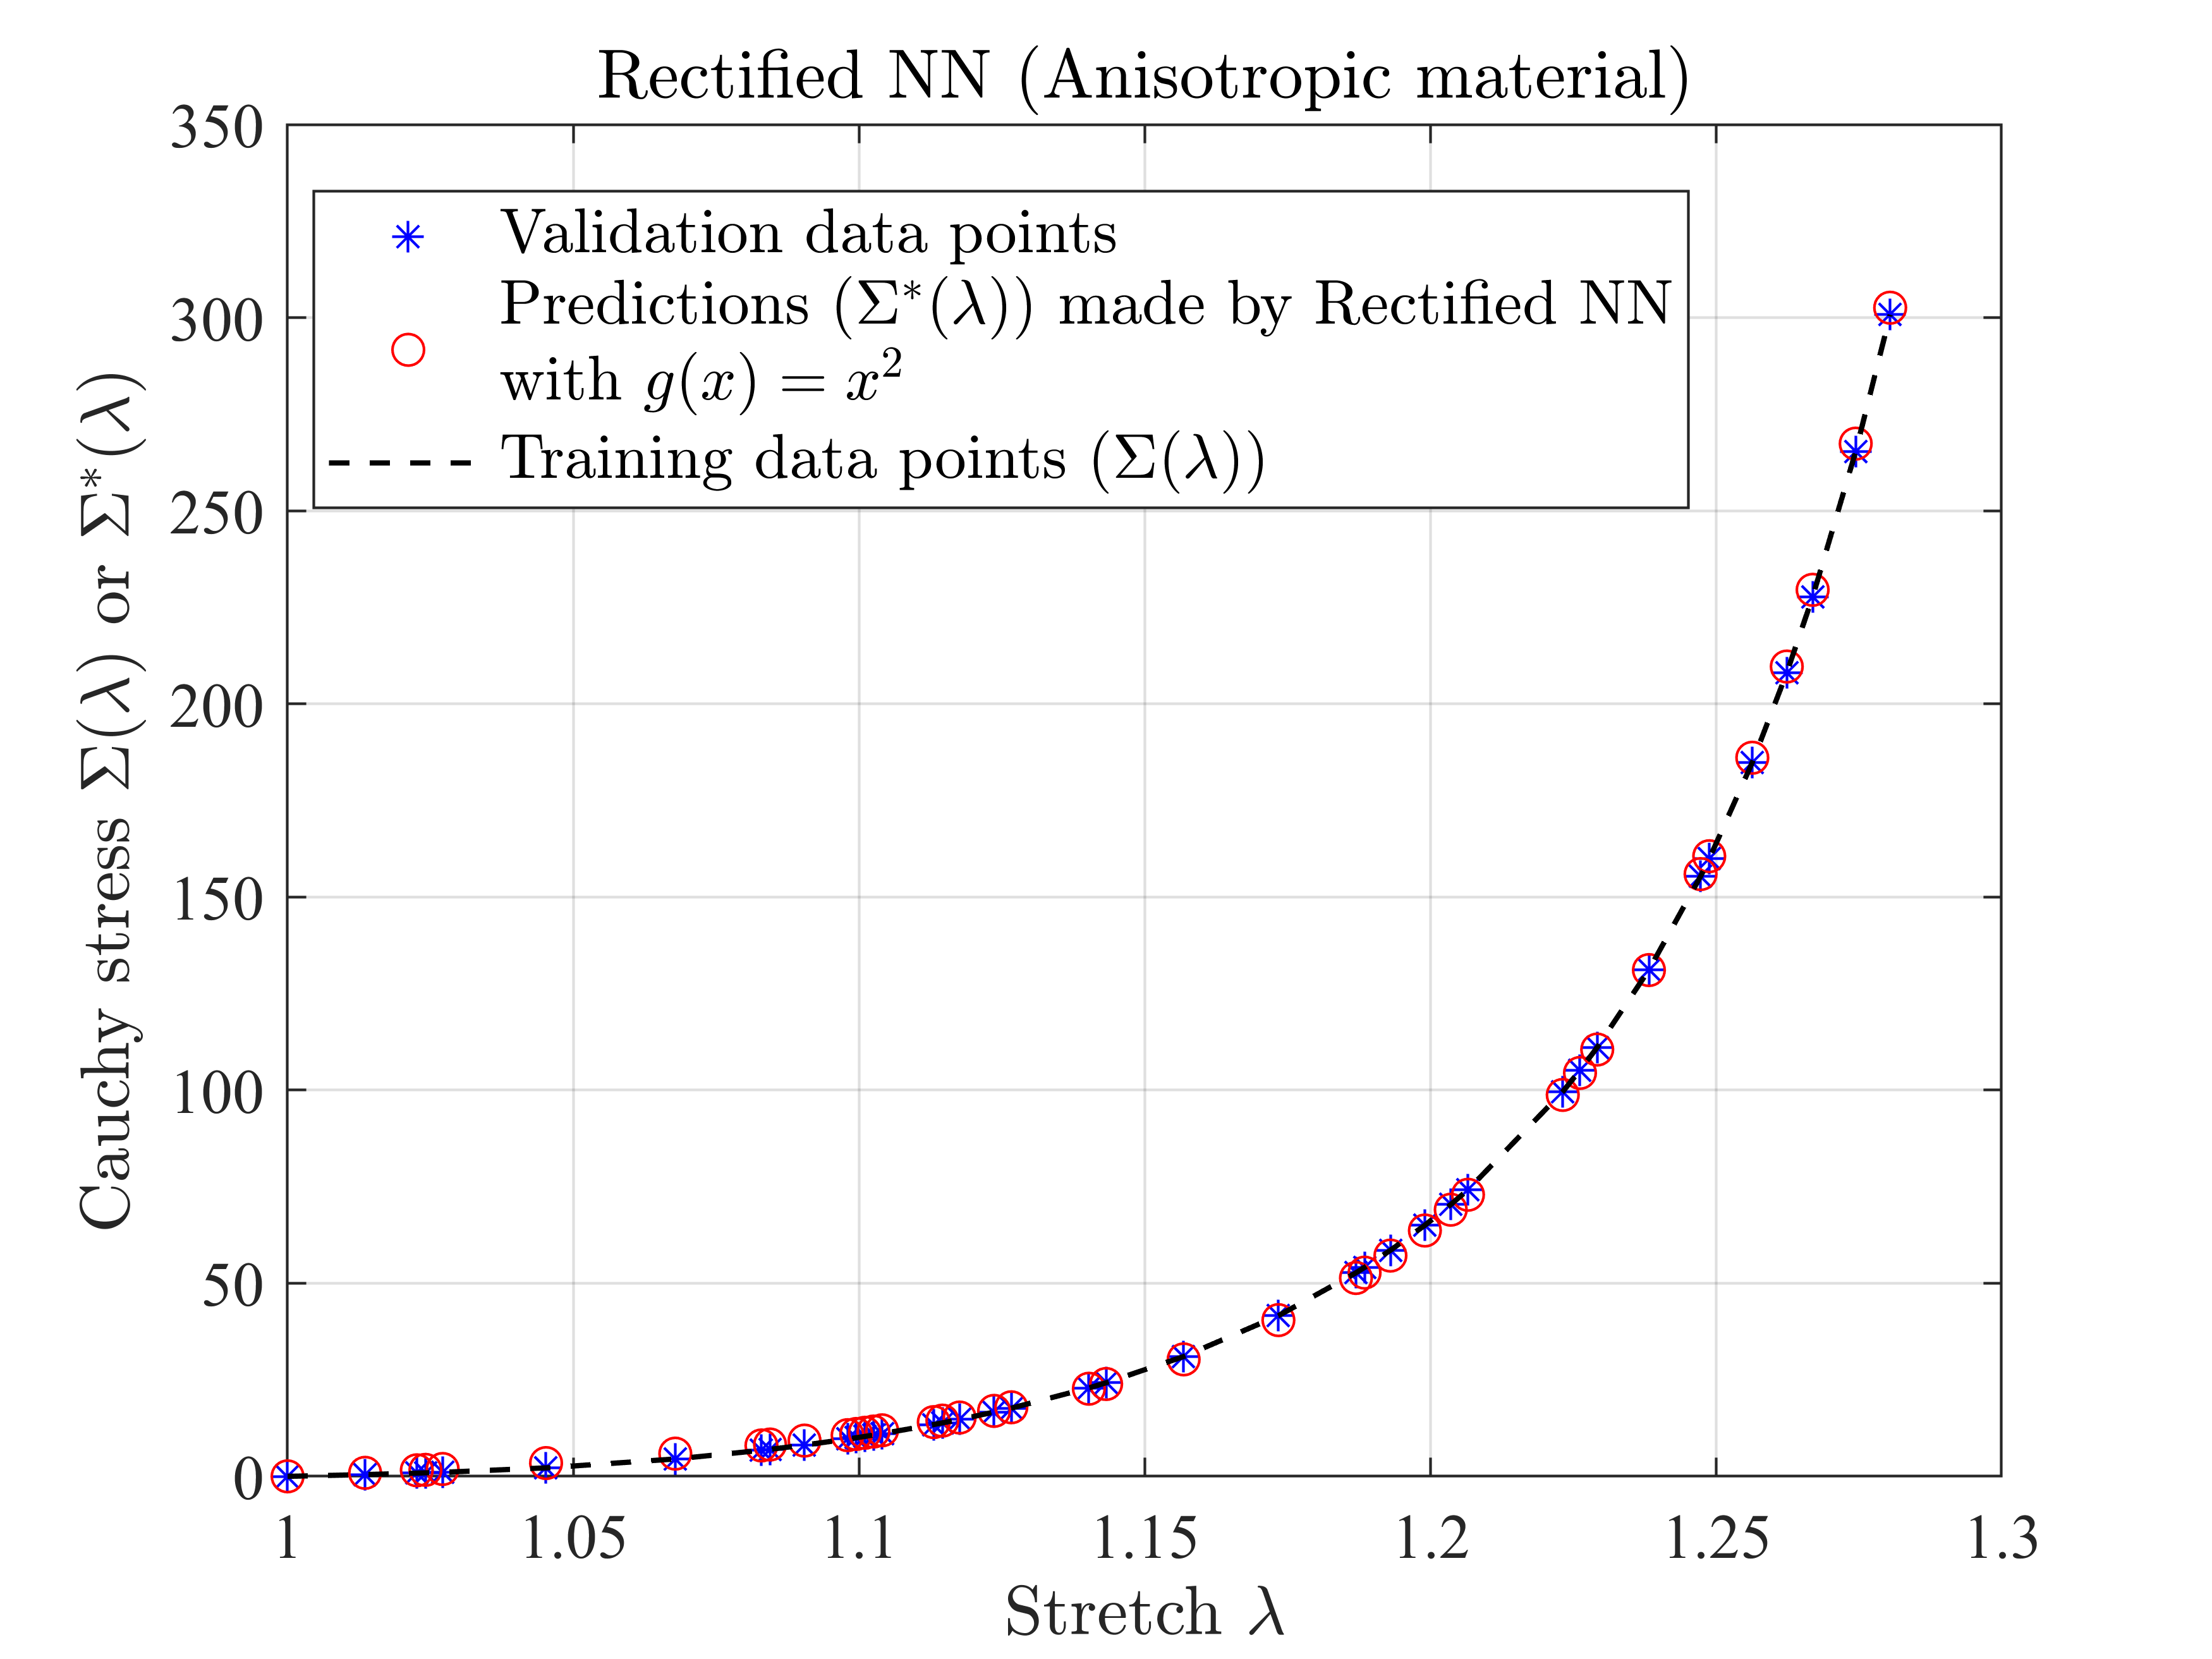
\includegraphics[width=0.5\textwidth]{Pictures/sigma_ANI.png}
    \end{center}
    \caption[Reference stress response $\lambda \mapsto \Sigma(\lambda)$, reference values, and rectified neural network predictions.]{Reference stress response $\lambda \mapsto \Sigma(\lambda)$ (black dashed line), reference values (blue star), and rectified neural network predictions (red circle) for the validation dataset (random selection). Here, the NN involves 4 hidden layers and 40 neurons per layer.}
    \label{fig:ANI best result 1}
\end{figure}
The validation metric in this example is $3.46 \times 10^{-6}$.

\subsection{Anisotropic Model for Experimental Dataset}\label{subsec:exp-app}
We finally apply the proposed rectification method to the experimental dataset presented in \cite{holzapfel2005determination}, corresponding to uniaxial extension tests on human illiac arterial walls. In those experiments, two different strips were harvested along the circumferential and longitudinal directions on each specimen to capture anisotropic effects. For the sake of illustration, two samples are randomly selected as target data for each layer defining the artery (adventitia, media, intima), and 10\% of the data is used as the validation dataset. The rectified neural network is similar to the one used in Section \ref{subsec:anisotropic-app} (see Eq.~\eqref{eq:rec-model-anisotropic-case}). 

Both axial and circumferential tension data are used for training. The Cauchy stress for the rectified model defined by Eq.~\eqref{eq:rec-model-anisotropic-case} in the circumferential direction reads as in Eq.~\eqref{eq:ANI_Cauchy}, in which
\begin{align}
    &\Sigma_1^*(\lambda) = 2 \frac{\partial w_1^*}{\partial I_1} \left(\lambda^2 - \frac{1}{\lambda}\right)\,, \\
    &\Sigma_2^*(\lambda) = 2 \frac{\partial w_2^*}{\partial I_2} \left(\lambda - \frac{1}{\lambda^2}\right)\,, \\
    &\Sigma_3^*(\lambda) = 2 \lambda^2 \frac{\partial w_3^*(J_4^{(1)})}{\partial J_4^{(1)}} \cos^2(\alpha)\,,
    \\
    &\Sigma_4^*(\lambda) = 2 \lambda^2 \frac{\partial w_4^*(J_4^{(2)})}{\partial J_4^{(2)}} \cos^2(\alpha)\,.
\end{align}
for uniaxial elongation.

The Cauchy stress for the tissue contribution in the longitudinal direction involves the terms
\begin{equation}
    \Sigma_3^*(\lambda) = 2 \lambda^2 \frac{\partial w_3^*(J_4^{(1)})}{\partial J_4^{(1)}} \sin^2(\alpha)
\end{equation}
and
\begin{equation}
    \Sigma_4^*(\lambda) = 2 \lambda^2 \frac{\partial w_4^*(J_4^{(2)})}{\partial J_4^{(2)}} \sin^2(\alpha)\,.
\end{equation}
The loss function in terms of datapoints is then defined as
\begin{align}
    \mathcal{L}_d = & \frac{\sum_{i=1}^{n_p^c} \left( \Sigma^{\text{exp}}(\lambda_{1}^c) - \Sigma^{*}(\lambda_{1}^c; \bfp) \right)^2}{\sum_{i=1}^{n_p^c} \Sigma^{\text{exp}}(\lambda_{1}^c)^2}  \nonumber \\ 
    & + \frac{\sum_{i=1}^{n_p^a} \left( \Sigma^{\text{exp}}(\lambda_{1}^a) - \Sigma^{*}(\lambda_{1}^a; \bfp) \right)^2}{\sum_{i=1}^{n_p^a} \Sigma^{\text{exp}}(\lambda_{1}^a)^2}\,,
\end{align}
where the superscripts ``c'' and ``a'' refer to data obtained by stretching along the circumferential and axial directions, respectively, $n_p^c$ and $n_p^a$ are the associated numbers of datapoints. As in Section \ref{subsec:anisotropic-app}, the stress free constraint is enforced in a strong sense by shifting the Cauchy stress.

Predictions obtained with the rectified neural network can be qualitatively compared with reference values in Fig.~\ref{fig:exp_circ} and Fig.~\ref{fig:exp_axial}, while validation errors can be found in Tab.~\ref{tab:val-err}. In this application, we used 2 hidden layers per neural network and 100 neurons per hidden layer. The rectified NN is trained for 2,000 epochs with a learning rate set to 0.01, then for 2,000 epochs with a learning rate taken as 0.001, and finally for 2,000 epochs at a learning rate set to 0.0001. 
\begin{figure}[ht!]
    \begin{center}
        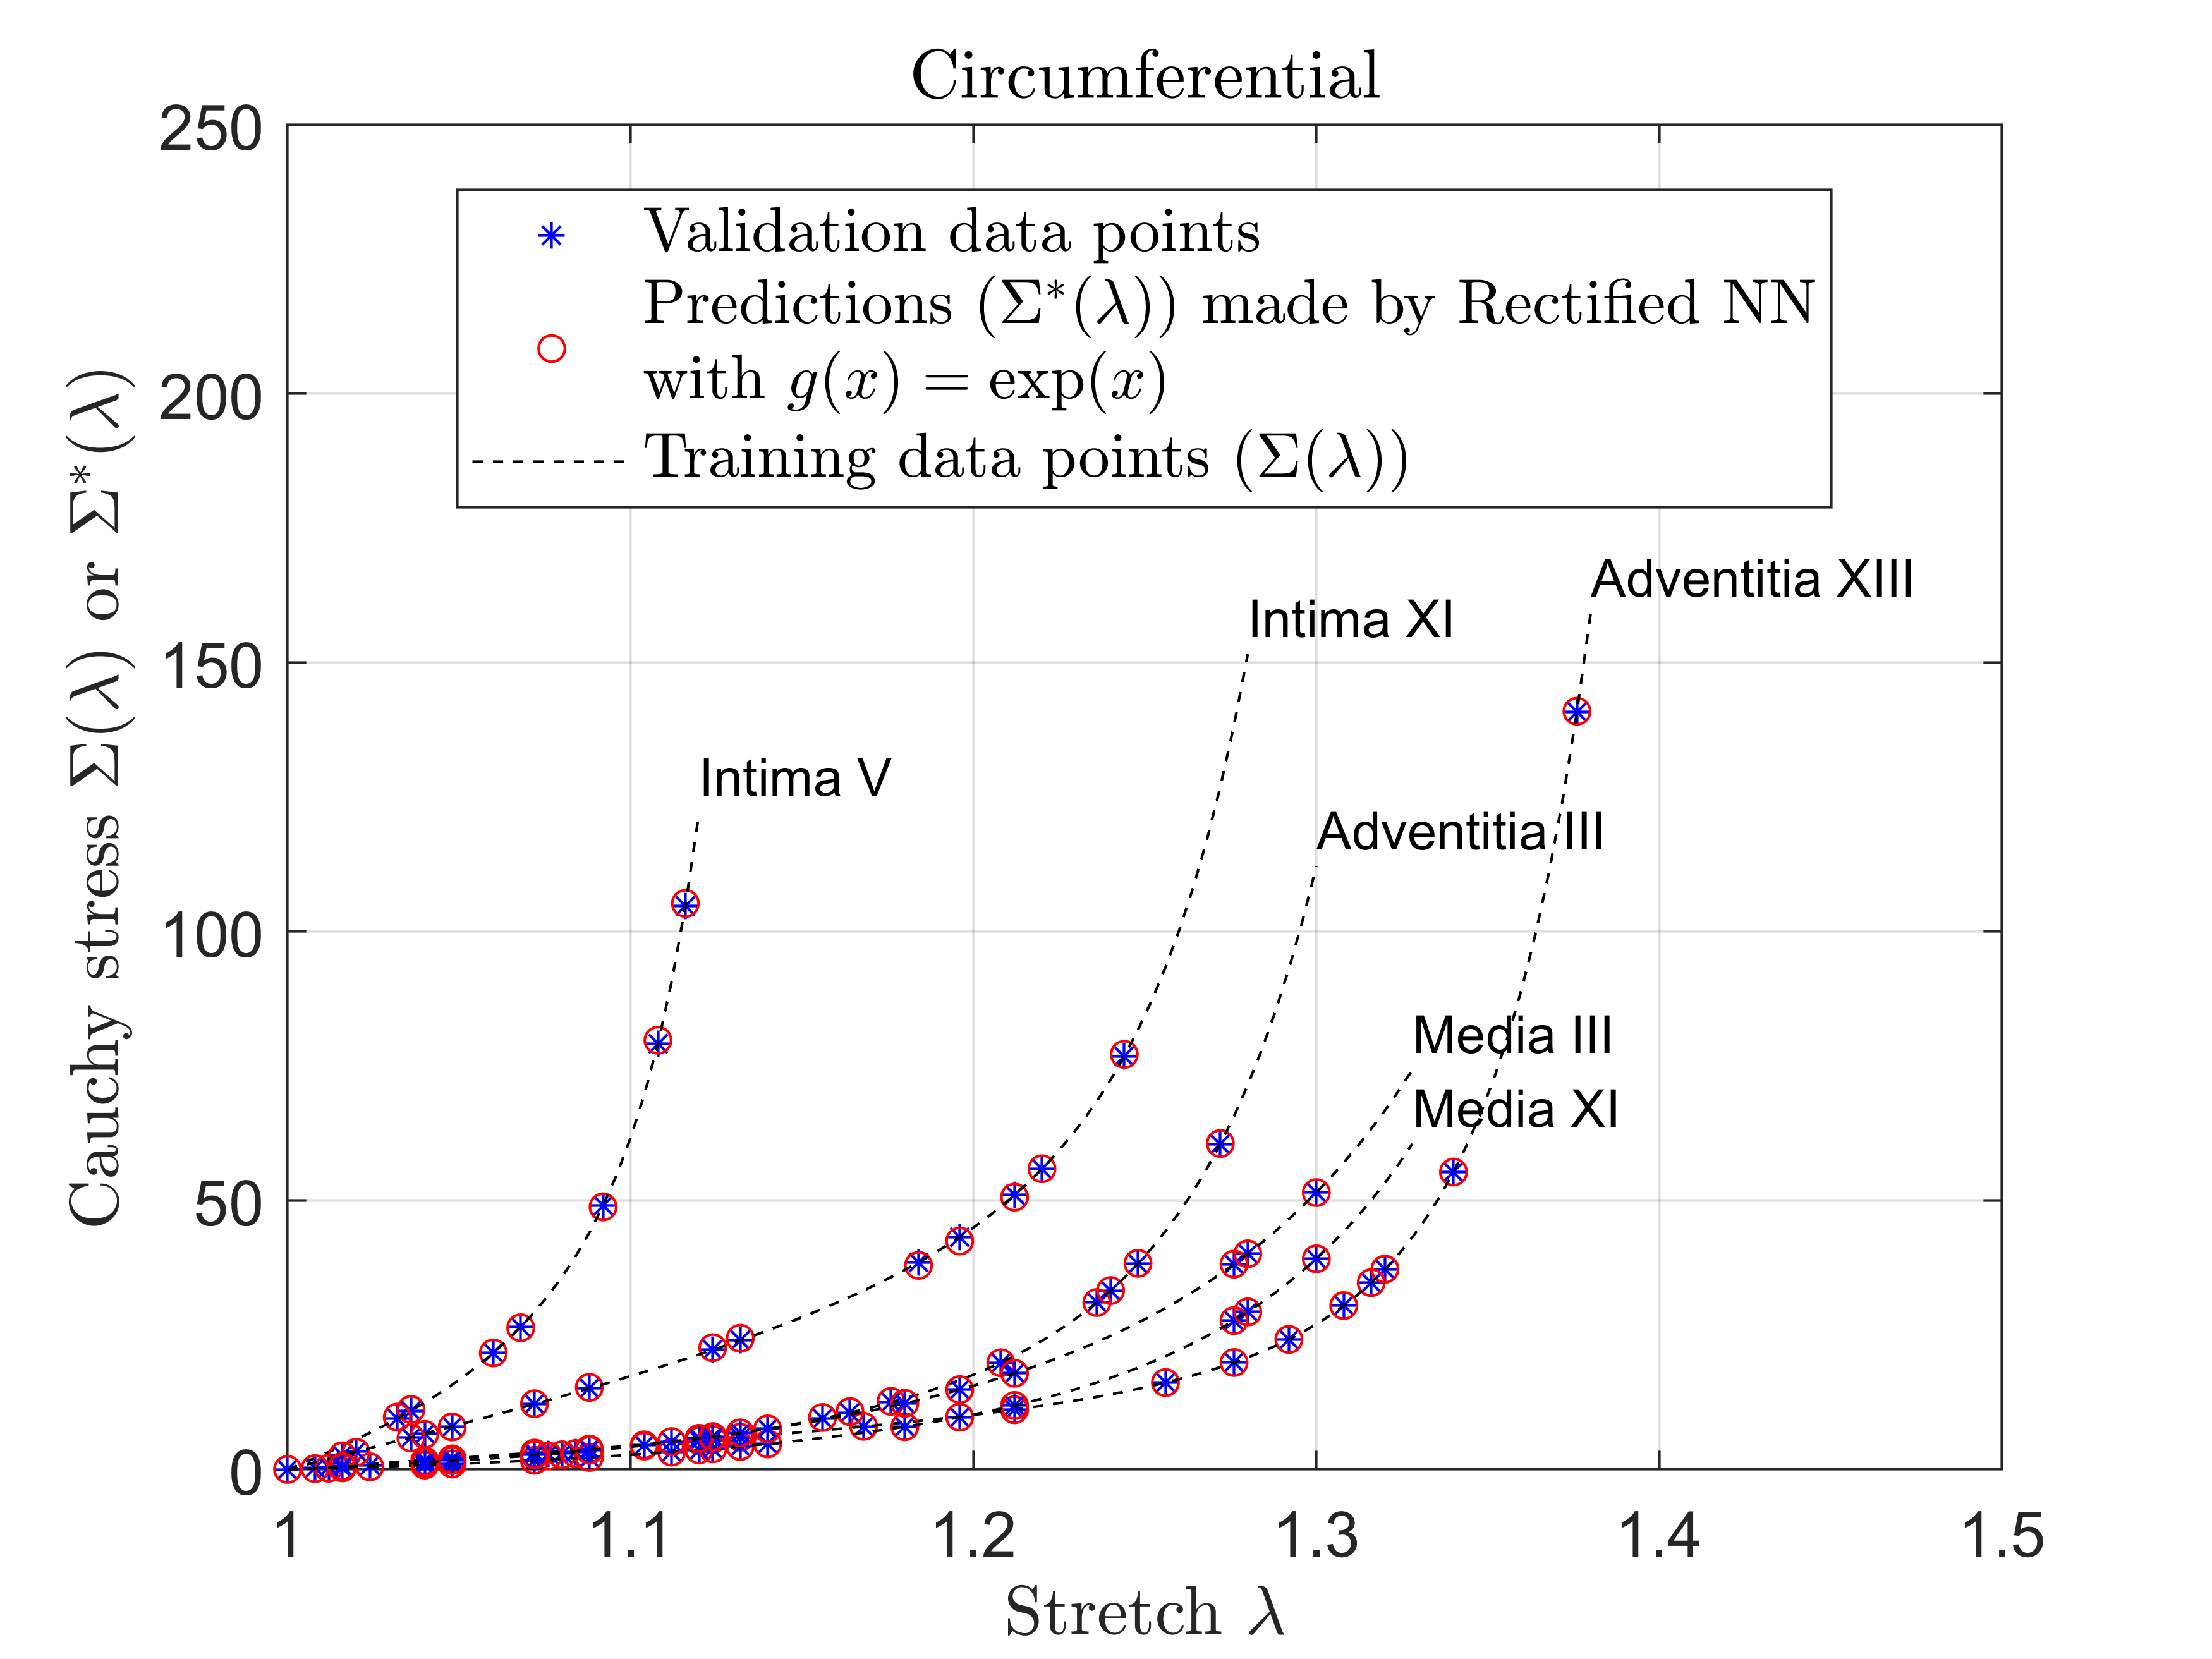
\includegraphics[width=0.5\textwidth]{Pictures/circ.png}
    \end{center}
    \caption[Reference stress response $\lambda \mapsto \Sigma(\lambda)$, reference values, and rectified neural network predictions in the circumferential direction.]{Reference stress response $\lambda \mapsto \Sigma(\lambda)$ (black dashed line), reference values (blue star), and rectified neural network predictions (red circle) for the validation dataset in the circumferential direction (six experimental responses are considered for illustration purposes).}
    \label{fig:exp_circ}
\end{figure}
\begin{figure}[ht!]
    \begin{center}
        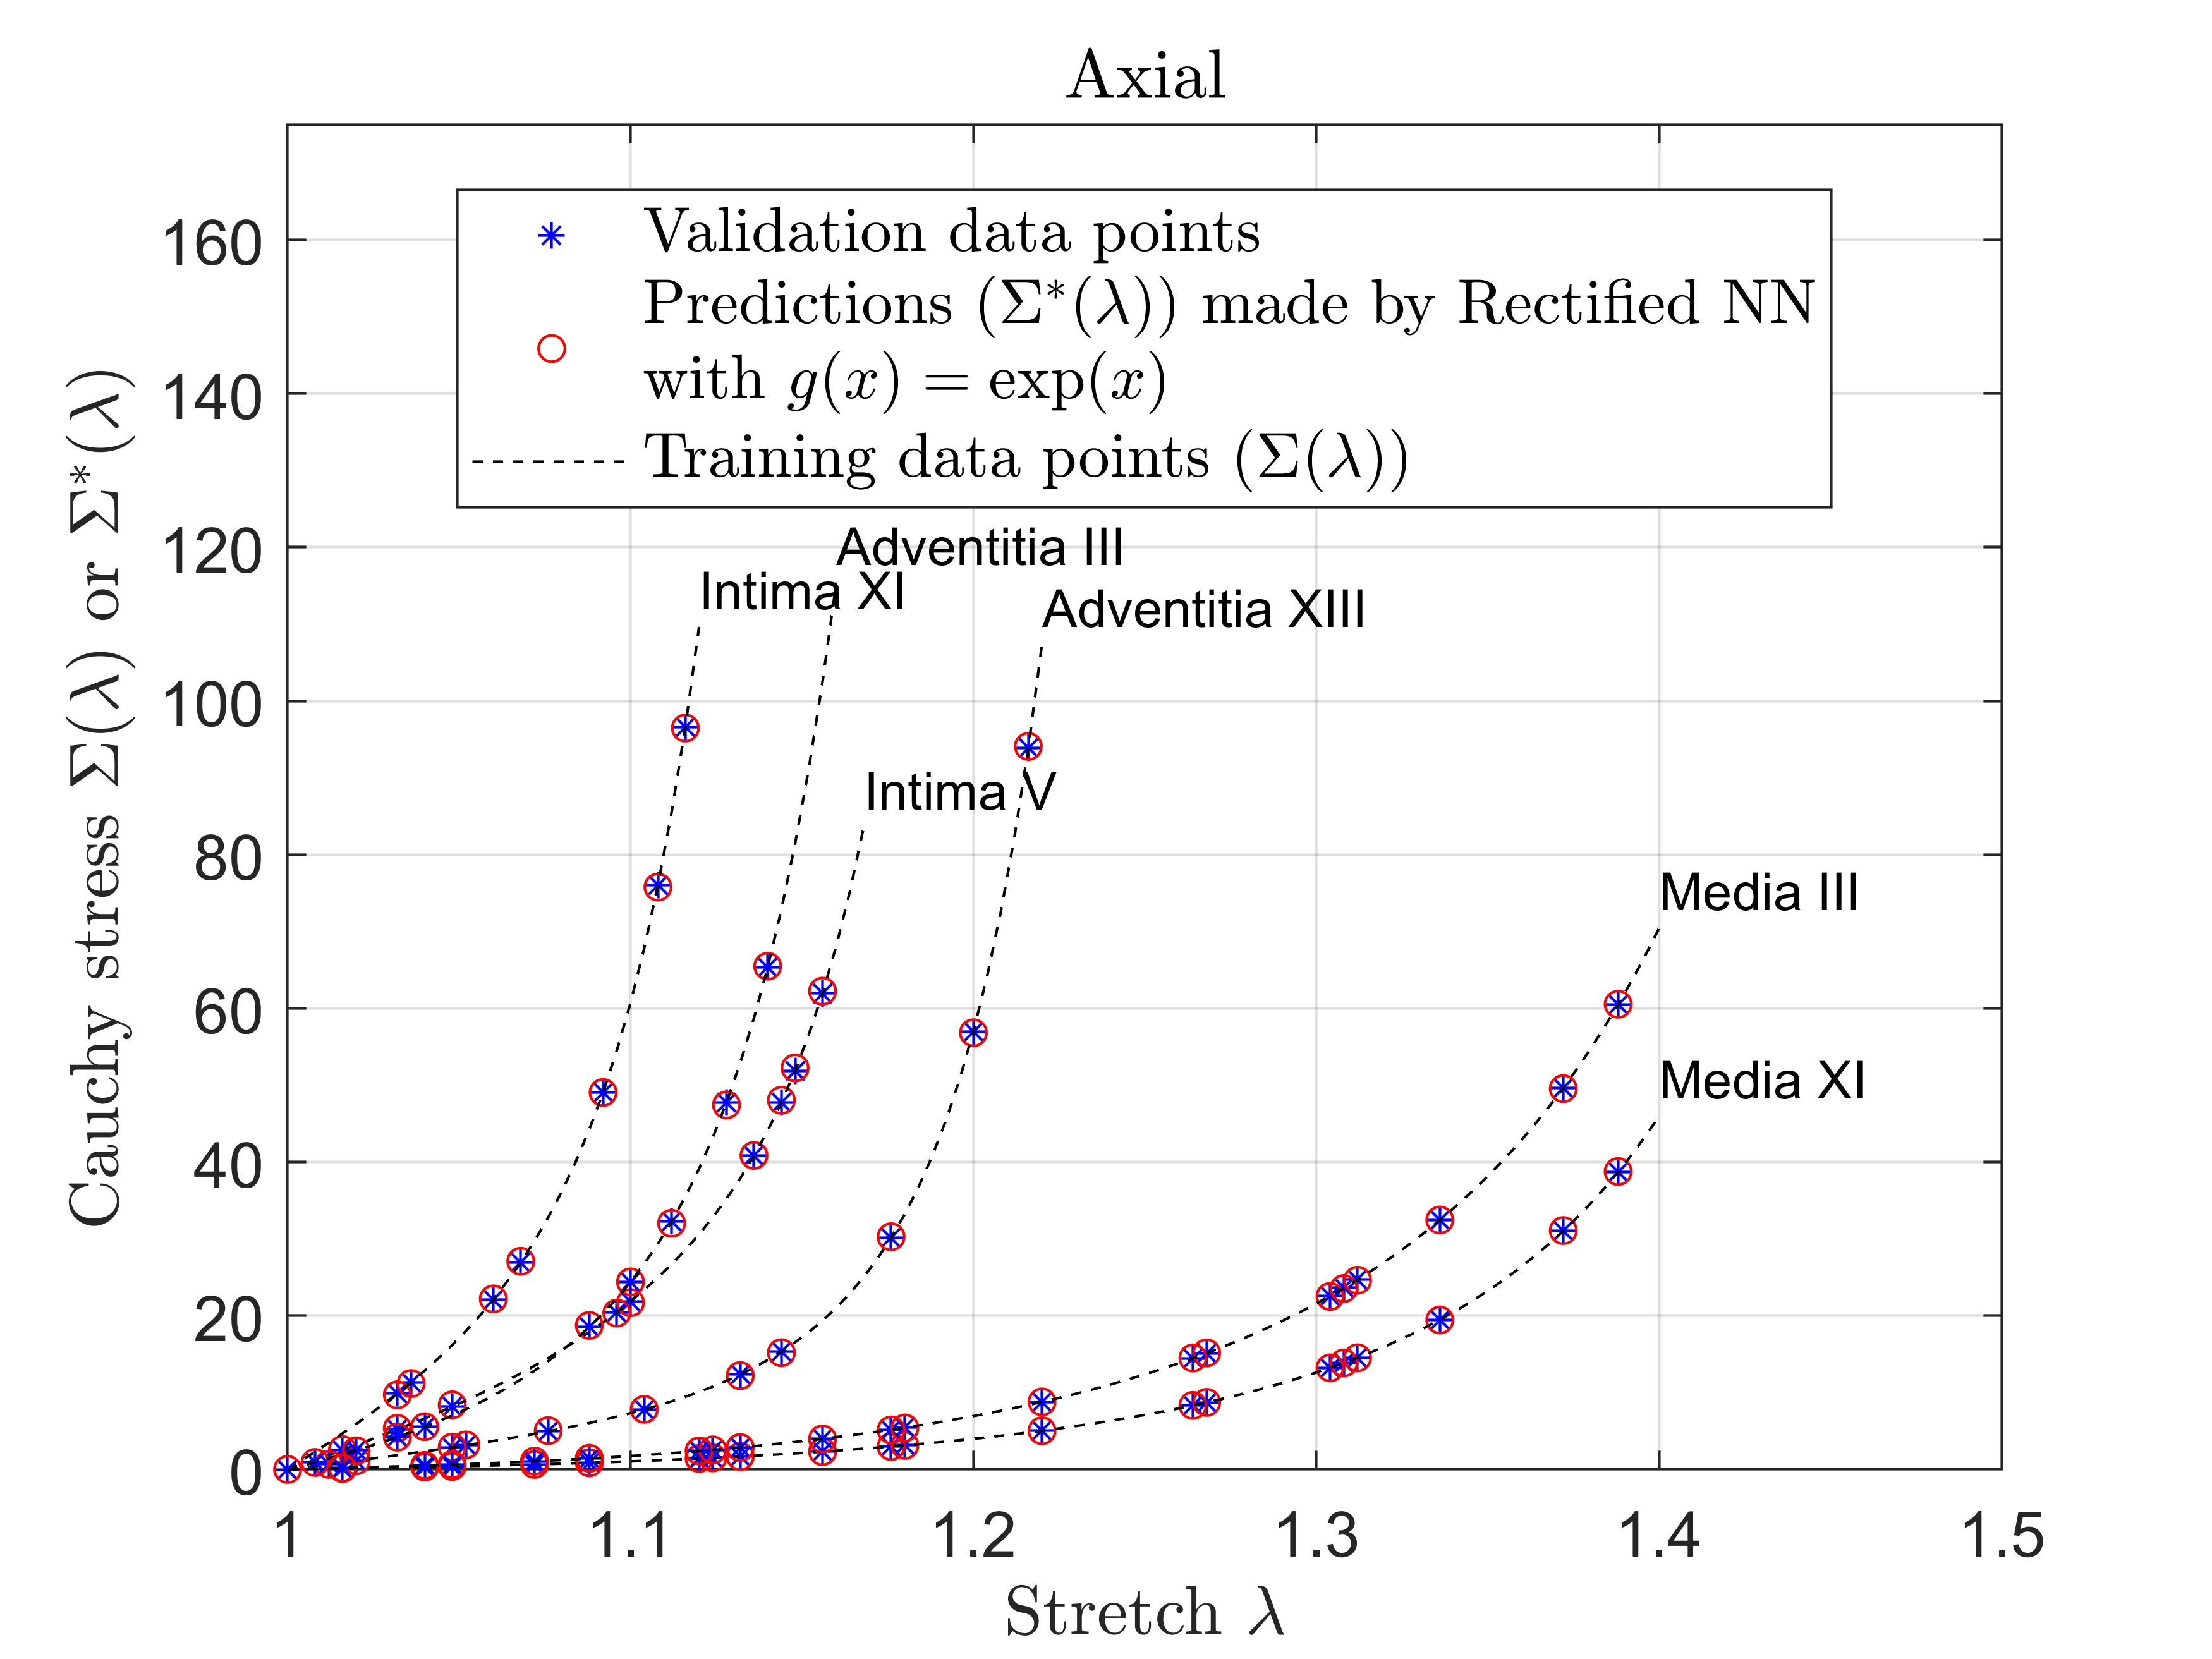
\includegraphics[width=0.5\textwidth]{Pictures/axial.png}
    \end{center}
    \caption[Reference stress response $\lambda \mapsto \Sigma(\lambda)$, reference values, and rectified neural network predictions in the axial direction.]{Reference stress response $\lambda \mapsto \Sigma(\lambda)$ (black dashed line), reference values (blue star), and rectified neural network predictions (red circle) for the validation dataset in the axial direction (six experimental responses are considered for illustration purposes).}
    \label{fig:exp_axial}
\end{figure}
With a maximal validation error equal to $1.0096\times10^{-4}$ (obtained for sample \#XI, intima layer), it is seen that the rectified neural network can reproduce the experimental data very well, for all different layers in the two directions.

\begin{table}[ht!]
\caption[Validation errors for each sample.]{Validation errors for each sample. Specimen numbers are those reported in \cite{holzapfel2005determination}.}
\label{tab:val-err}
\begin{center}
    \begin{tabular}{|c|c|} 
 \hline
 Layer/Specimen number & Error $\mathcal{L}_d$ $\times 10^{-4}$ \\
 \hline
 Adventitia/\#III & 0.9972 \\
 Adventitia/\#XIII & 0.1331 \\
 Intima/\#V & 0.7994 \\
 Intima/\#XI & 1.0096 \\
 Media/\#III & 0.0252 \\
 Media/\#XI & 0.0355 \\
 \hline
\end{tabular}
\end{center}

\end{table}
